\documentclass[11pt]{article}
\usepackage[T1]{fontenc}
\usepackage{lmodern}
\usepackage[margin=1.05in]{geometry}
\usepackage{amsmath,amssymb,amsthm,mathtools,mathrsfs}
\usepackage{microtype,booktabs,enumitem,graphicx,placeins}
\usepackage{tikz}
\usetikzlibrary{arrows.meta,positioning,calc,patterns}
\usepackage[hidelinks]{hyperref}
\hypersetup{pdftitle={The spherical magnetization law for the three-dimensional quantum Heisenberg ferromagnet},pdfauthor={OpenAI}}
\pdftrailerid{}
\numberwithin{equation}{section}
\allowdisplaybreaks[2]
\setlength{\emergencystretch}{2em}
\setcounter{tocdepth}{1}
\newtheorem{theorem}{Theorem}[section]
\newtheorem{proposition}[theorem]{Proposition}
\newtheorem{lemma}[theorem]{Lemma}
\newtheorem{corollary}[theorem]{Corollary}
\theoremstyle{definition}
\newtheorem{definition}[theorem]{Definition}
\theoremstyle{remark}
\newtheorem{remark}[theorem]{Remark}
\newcommand{\R}{\mathbb R}
\newcommand{\C}{\mathbb C}
\newcommand{\Z}{\mathbb Z}
\newcommand{\N}{\mathbb N}
\newcommand{\E}{\mathbb E}
\newcommand{\PP}{\mathbb P}
\newcommand{\1}{\mathbf1}
\newcommand{\dd}{\,\mathrm d}
\newcommand{\abs}[1]{\lvert#1\rvert}
\newcommand{\norm}[1]{\lVert#1\rVert}
\newcommand{\ip}[2]{\langle#1,#2\rangle}
\DeclareMathOperator{\Tr}{Tr}
\DeclareMathOperator{\diag}{diag}
\DeclareMathOperator{\dist}{dist}
\DeclareMathOperator{\supp}{supp}
\DeclareMathOperator{\diam}{diam}
\DeclareMathOperator{\rad}{rad}
\DeclareMathOperator{\Div}{div}
\DeclareMathOperator{\Rea}{Re}
\DeclareMathOperator{\Ima}{Im}
\DeclareMathOperator{\Var}{Var}
\DeclareMathOperator{\sech}{sech}
\newcommand{\articleid}[1]{\begingroup\small\ttfamily\hyphenchar\font=45 #1\endgroup}
\title{The spherical magnetization law for the\linebreak three-dimensional quantum Heisenberg ferromagnet}
\author{OpenAI}
\date{October 5, 2026}
\begin{document}
\maketitle
\begin{abstract}
We prove the spherical magnetization law for the three-dimensional
nearest-neighbor isotropic quantum Heisenberg ferromagnet at every fixed
positive quantum spin and every sufficiently low fixed positive
temperature. As the even periodic cubes grow, the symmetric zero-field
magnetization converges in moments to a uniform direction with a
deterministic positive magnitude. This magnitude equals the right
derivative at zero field of the infinite-volume pressure. The law is
expressed through self-adjoint linear combinations of the spin components
and requires no joint measurement of noncommuting observables.
\end{abstract}
\tableofcontents
\section{Introduction}\label{sec:introduction}

An isotropic ferromagnet has no preferred direction in zero field.
In a finite periodic volume, its Gibbs state is therefore rotation
invariant even at temperatures where magnetized equilibrium states exist.
The natural description of the ordered phase is a magnetization of fixed
length and uniformly distributed direction. Rotation invariance alone
does not establish this description: it allows a mixture of different
lengths. The question addressed here is whether the symmetric finite-volume
state selects a single length, and whether that length is the
magnetization selected by an infinitesimal field.

\subsection{Model and result}
Fix $S\in\{\tfrac12,1,\tfrac32,\ldots\}$. Let $S^1,S^2,S^3$ be the
irreducible spin-$S$ matrices, normalized by
\[
 [S^a,S^b]=i\sum_c\epsilon_{abc}S^c,
 \qquad \sum_{a=1}^3(S^a)^2=S(S+1)I.
\]
For even $L\ge4$, write $\Lambda_L=(\Z/L\Z)^3$ and $V=L^3$. On
$\bigotimes_{x\in\Lambda_L}\C^{2S+1}$, consider
\begin{equation}\label{eq:model}
 H_{S,L}=-\sum_{\{x,y\}\text{ nearest neighbors}}
              \sum_{a=1}^3 S_x^aS_y^a,
 \qquad M_L^a=\sum_{x\in\Lambda_L}S_x^a,
\end{equation}
where each unordered bond is counted once. We use the Gibbs expectation
\[
 \langle A\rangle_{\beta,L}
 =\frac{\Tr(Ae^{-\beta H_{S,L}})}{\Tr e^{-\beta H_{S,L}}}.
\]
The pressure and its right derivative at zero field are
\begin{align}
 p_{S,\beta}(h)
   &=\lim_{\substack{L\to\infty\\L\text{ even}}}
       \frac1{\beta V}\log\Tr
          e^{-\beta(H_{S,L}-hM_L^3)},\label{eq:pressure}\\
 m_{S,\beta}&=p_{S,\beta}'(0+).
       \label{eq:magnetization}
\end{align}
The pressure limit exists for this bounded finite-range interaction, and
convexity gives the right derivative. The volume limit in
\eqref{eq:pressure} precedes removal of the field.

\begin{theorem}[Spherical magnetization law]\label{thm:main}
For each fixed $S$ there is a finite $\beta_0(S)$ such that, for every
fixed finite $\beta\ge\beta_0(S)$, one has $m=m_{S,\beta}>0$ and
\begin{equation}\label{eq:spherical-law}
 \lim_{\substack{L\to\infty\\L\text{ even}}}
  \left\langle
     \exp\!\left(\frac1V\sum_{a=1}^3t_aM_L^a\right)
  \right\rangle_{\beta,L}
   =\frac1{4\pi}\int_{\mathbb S^2}e^{m t\cdot n}\dd\sigma(n)
   =\frac{\sinh(m|t|)}{m|t|}
 \qquad(t\in\R^3).
\end{equation}
Here $\sigma$ is surface-area measure on $\mathbb S^2$, and the quotient
at $t=0$ is interpreted as $1$. In addition,
\begin{equation}\label{eq:second-moment-law}
 \lim_{\substack{L\to\infty\\L\text{ even}}}
   \frac1{V^2}\sum_{x,y\in\Lambda_L}
          \langle S_x\cdot S_y\rangle_{\beta,L}=m^2.
\end{equation}
\end{theorem}

The statement uses self-adjoint linear combinations of the spin
components. It requires no joint finite-volume measurement of these
noncommuting operators. Both the spin and the positive temperature remain
fixed throughout the volume limit.

\subsection{Context and antecedents}\label{subsec:history}
The dimensional distinction in this problem is fundamental. Mermin and
Wagner~\cite{MerminWagner1966} excluded spontaneous ferro- or
antiferromagnetic order at positive temperature for finite-range
isotropic Heisenberg models in dimensions one and
two. In higher dimensions, infrared bounds proved continuous-symmetry
breaking for classical models~\cite{FSS1976} and ordering for quantum
antiferromagnets~\cite{DLS1978}. These quantum antiferromagnetic results
do not supply the isotropic ferromagnetic ordering input used here.
Another line of work establishes the low-temperature free-energy
asymptotic predicted by spin-wave theory~\cite{CGS2015}. That asymptotic
concerns a different limit from the field derivative or the zero-field
magnetization distribution at a fixed positive temperature.

The spherical distribution itself has clear antecedents. Ueltschi's
description of three-dimensional loop models~\cite[Section~8.1]{Ueltschi2017}
derives the transform $\sinh(hm)/(hm)$ for the spin-$\tfrac12$
ferromagnet conditional on a conjectured Poisson--Dirichlet law for
macroscopic loops. Bj\"ornberg, Fr\"ohlich, and
Ueltschi~\cite[Theorem~2.1]{BFU2020} prove the spherical transform
for the complete-graph quantum Heisenberg model at arbitrary fixed spin.
Our setting has nearest-neighbor interactions on the three-dimensional
lattice. We prove its magnetization law without assuming a distribution
for macroscopic loop lengths.

The existence of spontaneous magnetization and the identification of its
zero-field distribution are distinct questions. The companion manuscript
\cite{Ord} constructs magnetized equilibrium states for the isotropic
nearest-neighbor quantum Heisenberg ferromagnet in dimensions at least
three, for every fixed spin at sufficiently low positive temperatures.
The companion \cite{BL} establishes the low-temperature asymptotic
of the pressure-defined magnetization for nonnegative symmetric
finite-range interactions whose support generates $\Z^3$.
We use finite exchange and geometric estimates from these works. The present
argument adds spatial control on periodic tori and a pressure argument
excluding translation-ergodic equilibrium states with different
magnetization magnitudes.

The exchange representation builds on permutation and random-walk
representations of quantum spins~\cite{Powers1976,ConlonSolovej1991Representation},
T\'oth's random-stirring representation~\cite{Toth1993}, and its
higher-spin formulation through symmetric slots~\cite{Nachtergaele1994}.
The finite pin estimates used below draw on the stability and negative
dependence theory of Borcea, Br\"and\'en, and Liggett~\cite{BBL2009}.
Our zero-free matrix products use the contraction principle associated
with Asano's and Ruelle's developments of Lee--Yang theory
\cite{Asano1970,Ruelle1971,Ruelle1973}; the contraction needed here is
proved explicitly. Mean entropy, equilibrium states, and pressure
tangents are treated within the variational framework of Lanford and
Robinson~\cite{LanfordRobinson1968Entropy,LanfordRobinson1968Spin}.
We recall the required facts and prove the additional replica and
harmonic-selection statements.

\subsection{The two parts of the proof}\label{subsec:strategy}
Here is the obstruction that the proof must overcome. Let $J_L$ denote the
total-spin label in the rotation-invariant Gibbs state. Conditional on
$J_L$, any component of $M_L$ is uniform on
$-J_L,-J_L+1,\ldots,J_L$. A fixed positive field and the definition of $m$
already imply
\begin{equation}\label{eq:overview-upper}
 \PP(J_L/V>m+\epsilon)\longrightarrow0
 \qquad(\epsilon>0).
\end{equation}
Thus it remains to prove
\begin{equation}\label{eq:overview-lower}
 \liminf_{L\to\infty}\frac{\E[J_L(J_L+1)]}{V^2}\ge m^2.
\end{equation}
Together these bounds force $J_L/V\to m$ in probability and give
\eqref{eq:spherical-law}. Section~\ref{sec:global-spin} supplies this
last representation-theoretic argument in detail.

Two facts produce the lower bound. First, the squared magnetization
averaged on large local boxes is controlled by the squared magnetization
averaged on the whole torus, with an error vanishing as the local scale
grows. This prevents local magnetization from canceling through spatial
variation on larger scales. Second, every translation-ergodic equilibrium
state has magnetization vector of length $m$. Here an equilibrium state
maximizes mean entropy minus $\beta$ times the physical energy density
among translation-invariant
states; an ergodic state is an extreme point of that invariant state
space. Their variational and averaging properties are recalled in
Section~\ref{sec:equilibrium}. The second fact identifies the local
magnetization length to which the first fact applies.

Both facts use the same weak exponential estimate. To describe it, let
$\mathcal P$ be a rectangular partition whose cell sides are comparable
to a large scale $R\le L$. For a deterministic site function $f$ with
$|f_x|\le1$ and $\sum_{x\in C}f_x=0$ in each cell, put
$D_f=\sum_xf_xS_x^3$. We prove, for
$b_R\asymp R^{-5/2}$ and a fixed $\kappa>0$, that
\begin{equation}\label{eq:overview-exp}
 \log\langle e^{\theta_R D_f}\rangle_{\beta,L}
       \le C_\beta b_R V,
 \qquad \theta_R=\kappa b_R\log R.
\end{equation}
In particular the left side divided by $\theta_R V$ tends to zero
uniformly in these tests. In nested rectangular partitions, apply this
bound to signs of differences between a cell average and its parent
average. A union bound and a telescoping identity then control all spatial
scales. Applied to a product of two local zero-sum spin tests in
different replicas, it forces the expectation of that product to vanish
in every equilibrium state of the replicated system: finite-volume
restrictions of such a state have relative entropy per site tending to
zero with respect to the product Gibbs state.

Obtaining \eqref{eq:overview-exp} is the spatial part of the proof.
Sections~\ref{sec:exchange}--\ref{sec:spatial-comparison} use exchange
cycles and a field of strength $b_R$ in a perpendicular direction to bound
$R^{-5/2}V^{-1}\langle D_f^2\rangle_{b_R}$ by a negative power of $R$.
The field gives a killed one-particle kernel an invertible resolvent.
A sparse-pin estimate controls the holes left after exposing unpinned
cycles; a comparison on this random set then uses the zero sum of $f$ in
each cell. Section~\ref{sec:zero-field} turns the resulting variance
bound into \eqref{eq:overview-exp} through a zero-free complex strip.

The remaining argument identifies the magnitude. Negative squares of
large-box magnetization averages would distinguish states of different
lengths, but the corresponding perturbed Gibbs operators do not directly
fit the exchange zero-freeness argument. Section~\ref{sec:pressure}
realizes these perturbations as first-order averages of random products
of real matrices acting on the $2S$ spin-$\tfrac12$ slots representing
each site. Let $Z(z)$ be the normalized trace of such a product with
complex field $z$. For every realization, $Z(z)$ is nonzero on
$\Rea z>0$. Shared Gaussian variables couple its moments to replicated
pressures; the zero-sum cross terms just described disappear from their
pressure derivatives. Moment bounds then select harmonic limits of
normalized $\log|Z(z)|$. Analyticity of their restrictions to
the real axis excludes coexistence of different ergodic magnetization
lengths. More concretely, an ergodic state of length $a$, oriented along
the auxiliary field, contributes the affine function $xa-a^2$ to a
limiting pressure tangent. Large positive $x$
selects the branch $xm-m^2$; analytic continuation of that branch cannot
dominate a competing branch of smaller length at every positive $x$.
The spatial estimate, the replica argument, and the passage from
random zero-free functions to harmonic pressure tangents are the main
additional constructions of this paper.

\subsection{Conventions}\label{subsec:conventions}
We suppress $S$ in expectations and usually suppress $\beta,L$ when no
confusion is possible. Write $X,Y,Z$ for the site spin components
$1,2,3$, in the standard representation where $X,Z$ are real and $Y$ is
imaginary. Set $H_0=-\beta H_{S,L}$. Constants $c,C$ may depend on the fixed
spin and on fixed geometric choices; $C_\beta$ may also depend on the
fixed inverse temperature. We first choose a sufficiently large finite
$\beta$, and only then choose lower thresholds for $L$ and spatial scales.
All torus volume limits are through even $L$.

The finite exchange inputs are developed in Section~\ref{sec:exchange},
and the deterministic lattice estimates imported from the companions
are stated with their hypotheses where they are used. Positivity of
$m$ follows directly from our torus sparse-pin estimate in
Corollary~\ref{cor:positive-magnetization}; no sharp low-temperature
asymptotic is needed. We increase $\beta_0(S)$ as needed below.

\section{Exchange cycles, pins, and zero-free traces}\label{sec:exchange}

The exchange representation gives two finite-dimensional tools for the
proof.  Pinning and exposing cycles turns a return probability into the
first moment of a Markov hitting kernel.  Stability of the same exchange
operators also gives zero-free traces after insertion of suitable
single-slot matrices.  We develop both tools here, keeping track of the
conditioning in the first and the trace contraction in the second.

\subsection{Symmetric slots and permutation layers}

Put $\ell=2S$ and let
$\mathcal I=\Lambda_L\times\{1,\ldots,\ell\}$ be the set of
$N=\ell V$ slots.  On $(\C^2)^{\otimes\mathcal I}$ write
$s_i^a$ for the Pauli matrices divided by two, and let
\[
 P_* =\prod_{x\in\Lambda_L}\frac1{\ell!}
                  \sum_{\pi\in\mathfrak S_\ell}\mathcal U_{\pi,x}
\]
be the projection onto the tensor product of the symmetric site
subspaces.  Here $\mathcal U_{\pi,x}$ permutes the slots at $x$.
On this subspace $S_x^a=\sum_{i:\,x_i=x}s_i^a$ is the spin-$S$
representation.  In particular, if compression is needed for an individual
slot operator, then
\begin{equation}\label{eq:compressed-slot}
        P_*s_i^aP_* = \ell^{-1}S_{x_i}^aP_*.
\end{equation}

For each site bond use all $\ell^2$ slot edges above it.  On these
edges put independent Poisson exchanges of rate $1/2$ during
$[0,\beta)$, and at the seam from $\beta$ to $0$ insert an independent
uniform slot permutation at every site.  Let $\pi$ be the resulting
permutation of $\mathcal I$ and $\mathbb P_{\rm b}$ its underlying
picture law.  If $\mathcal E$ is the set of slot edges, then
\begin{equation}\label{eq:exchange-operator}
 e^{H_0}P_*=e^{\beta|\mathcal E|/4}
                    \E_{\rm b}\mathcal U_\pi,
 \qquad H_0=-\beta H_{S,L}.
\end{equation}
On the left $H_0$ is lifted to the slot space before compression.
Indeed,
$\boldsymbol s_i\cdot\boldsymbol s_j=\frac12\mathcal U_{(ij)}-\frac14I$,
and the mean chronological Poisson product has generator
$\frac12\sum_{e\in\mathcal E}(\mathcal U_e-I)$.
The all-slot sum above each bond commutes with $P_*$, while the seam
average inserts $P_*$.  This proves \eqref{eq:exchange-operator}.
This is T\'oth's exchange representation \cite{Toth1993}, with the
higher-spin construction of Nachtergaele
\cite[Section~2.2]{Nachtergaele1994}; see also
\cite[Proposition~2.1]{BL}.

If $A$ is a polynomial in the physical site spins, let $\widehat A$
be its slot lift obtained by replacing $S_x^a$ by
$\sum_{i:\,x_i=x}s_i^a$.  The physical trace is then
\begin{equation}\label{eq:physical-slot-trace}
       \Tr_{\rm phys}(Ae^{H_0})
          =\Tr_{\rm slot}(\widehat A e^{H_0}P_*).
\end{equation}
Following lines through repetitions of one sampled picture gives its
cycles.  In this slot trace with diagonal spin insertions a cycle has a constant
up or down color.  Without insertions its contribution is two.  We take
slot-time points immediately after an instantaneous operation, including
the seam.  In finite volume there are almost surely finitely many marks,
with distinct times avoiding any prescribed finite set of cuts.

We call a permutation law on a finite set \emph{admissible} if it is a
distributional limit of finite products of independent Bernoulli
transpositions and deterministic permutations.  Products here are ordered;
no commutation is assumed.  This class includes finite-time Poisson
exchanges at arbitrary nonnegative rates, uniform permutations on
specified subsets, and independent compositions of these operations.
For the Poisson assertion, divide time into small intervals and apply
each edge's Bernoulli indicator of at least one mark in a fixed order.
The approximation agrees with the picture unless an interval contains
at least two marks, whose probability tends to zero.  For a uniform
permutation, run positive-rate exchanges on every pair of the given
subset and let time tend to infinity.  This irreducible random walk on
the finite permutation group converges to its uniform invariant law.

We use the following finite stability facts.  A nonzero polynomial is
\emph{stable} if it does not vanish when all variables have positive
imaginary parts.  For every admissible law of a permutation $\pi$ of a
finite set $I$,
\begin{equation}\label{eq:stable-permutation-symbol}
              \E\prod_{i\in I}(u_i+v_{\pi(i)})
                    \quad\hbox{is stable}.
\end{equation}
Identification of variables preserves stability; differentiation, real
specialization, and bounded-degree coefficientwise limits preserve it
up to the zero polynomial.  Finally, if a random subset $A\subseteq I$
has a stable generating polynomial
$G_A(\boldsymbol z)=\E\prod_{j\in A}z_j$, then for every $J\subseteq I$,
\begin{equation}\label{eq:stable-presence}
            \Pr(J\subseteq A)\le\prod_{j\in J}\Pr(j\in A).
\end{equation}
These are the partial-symmetrization and negative-dependence facts in
\cite[Theorems~4.20 and~4.9]{BBL2009}; the exact finite formulations
and their elementary proofs appear in \cite[Lemmas~3.2--3.6]{Ord}.
In particular, the facts apply on a disjoint union of time layers,
without any spatial assumptions.

\subsection{Pins and exposure}

The finite constructions in this subsection allow independent Poisson
exchanges on an arbitrary finite slot graph, together with finitely many
prescribed deterministic permutations, Bernoulli transpositions, and
uniform permutations on prescribed subsets at fixed times.  All random operations are
independent under the base law.  Their order at
coincident prescribed times is fixed, and a slot-time point at such a
time lies after the entire ordered bundle of operations.  Thus extra stationary lines and
extra instantaneous exchanges are included.

A \emph{pin} is a specified slot-time point required to have up color.
For a finite deterministic pin set $E$, let $n_E$ be the number of
cycles avoiding $E$, let $\mathcal B_E$ be their union, and define
\begin{equation}\label{eq:pin-law}
 \mathcal Z_E=\E_{\rm b}2^{n_E},\qquad
       \mathbb P_E(d\omega)
         =\mathcal Z_E^{-1}2^{n_E(\omega)}\mathbb P_{\rm b}(d\omega).
\end{equation}
Cycles meeting pins are up; the others are colored independently and
fairly.  For a nonempty single-time set $T$ disjoint from $E$, put
$P=E\cup T$ and let $\sigma$ take each pin in $P$ to the next pin
on its directed cycle, at strictly positive elapsed time.  Set
\begin{equation}\label{eq:pin-return}
       r(E,T)=\frac1{|T|}\sum_{i\in T}
                              \mathbb P_P\{\sigma(i)\in T\}.
\end{equation}
The same sampled picture is repeated in defining $\sigma$.

To describe exposure, label lines at time zero and reveal all labels on
cycles missing $P$, their trajectories through a period, and all their
endpoint images.  The trajectories record their positions before and
after each elementary operation, including intermediate stages of an
ordered bundle at one time.  Denote these data by $\mathbf a$.  The slots not
occupied by exposed labels are called \emph{holes}.  For fixed exposure,
define a fresh law $\mathbb Q_{\mathbf a}$ on the holes as follows.
Exchanges whose two endpoints are holes have their original independent
Poisson clocks.  At a transposition exchanging an exposed label with a
hole, that hole moves into the vacated slot.  These forced transports are deterministic
bijections between successive hole layers.  A partly revealed uniform
permutation is completed by a uniform bijection between the remaining
source and target slots; a prescribed deterministic permutation restricts
to a deterministic bijection between those hole layers.
An elementary Bernoulli transposition touching
an exposed label has its outcome revealed; one touching only holes
retains its independent Bernoulli law.  Let $G_P$ denote the event that
every cycle of this fresh picture meets $P$.

\begin{lemma}[Finite pin inputs]\label{lem:pin-inputs}
For the finite picture above the following assertions hold.
\begin{enumerate}[label=(\roman*),leftmargin=*]
\item For every finite $E$ and nonempty single-time $T$ disjoint from $E$,
\begin{equation}\label{eq:simultaneous-pin}
                  \mathbb P_E(T\subseteq\mathcal B_E)
                                  \le(2r(E,T))^{|T|}.
\end{equation}
\item Almost surely under $\mathbb P_P$,
$g_P(\mathbf a):=\mathbb Q_{\mathbf a}(G_P)>0$, and the conditional
law of the remaining picture is
$\mathbb Q_{\mathbf a}(\,\cdot\mid G_P)$.
\item Let $\omega_{\rm m}$ be the Poisson mark counting measure and
let $\lambda_{\rm b}$ be edge rate times Lebesgue time measure.
For every integer $j\ge1$
and nonnegative measurable function $F$ of $j$ mark locations,
\begin{equation}\label{eq:factorial-domination}
 \E_E\sum_{(u_1,\ldots,u_j)\in\omega_{\rm m,\ne}^j}
                F(u_1,\ldots,u_j)
       \le 2^j\int F\,d\lambda_{\rm b}^{\otimes j}.
\end{equation}
The sum is over ordered distinct marks, and may be restricted to any
prescribed time order.  Independent additional fresh Poisson clocks
may be included with their own, undoubled, factorial intensity.
\end{enumerate}
\end{lemma}

\begin{proof}
The statements are the finite-pin forms of
\cite[Proposition~2.4, Proposition~2.5, and Lemma~2.3]{BL}.
We give the arguments to specify the scope of the extra operations and
the measure used after exposure.

Cut at all pin times and at zero, and let $\mathcal V$ be the disjoint
union of the slot layers at these cuts.  The maps between successive
cuts are independent admissible bijections.  Their symbols in disjoint
input and output variables multiply to give a stable polynomial
$\E_{\rm b}\prod_{i\in\mathcal V}(x_i+y_{\pi(i)})$.
Delete a nonpin $q$ by setting $x_q=y_q=t$ and extracting the
coefficient of $t$.  If its predecessor and successor are $i,j$, then
$(x_i+t)(t+y_j)$ is replaced by $x_i+y_j$.  A fixed point instead
contributes $2t$, hence a factor two.  Successive deletion therefore
gives the nonzero stable polynomial
\[
       \E_{\rm b}\left[2^{n_P}
                         \prod_{i\in P}(x_i+y_{\sigma(i)})\right].
\]
Differentiate in the input variables indexed by $P\setminus T$, set
all input variables to zero, and divide by $\mathcal Z_P$.
The result is
$\E_P\prod_{i\in T}y_{\sigma(i)}$, the stable generating polynomial
of the subset $\sigma(T)$.  By \eqref{eq:stable-presence} and the arithmetic--geometric
mean inequality,
\[
 \mathbb P_P\{\sigma(T)=T\}
  \le\prod_{j\in T}\mathbb P_P\{j\in\sigma(T)\}
  \le r(E,T)^{|T|}.
\]
Here $\sum_{j\in T}\mathbb P_P\{j\in\sigma(T)\}=|T|r(E,T)$
by bijectivity.  The event $\sigma(T)=T$ is precisely
$T\subseteq\mathcal B_E$: iterating the next-pin permutation from
$T$ then meets no pin in $E$.  Finally,
$2^{n_P}\le2^{n_E}\le2^{|T|}2^{n_P}$ and
$\mathcal Z_E\ge\mathcal Z_P$, proving (i).

For (ii), first fix a proposed set $A$ of initial exposed labels.
Use two independent Poisson clock families on every edge, each with
the original rate: accept the first family's clock when an endpoint
contains an $A$-label and the second when neither does.  This realizes
the base process.  Given the past, the superposed clock has twice the
total original rate, each edge is accepted with its original relative
rate, and the rejection probability is $1/2$.  The $A$-label paths
use only the first family.  Given these paths, the second family
restricted to the hole intervals remains fresh.  Revealing the
$A$-label images at a uniform permutation leaves a uniform residual
bijection.  At a Bernoulli transposition its outcome is revealed
exactly when an exposed label is involved; other outcomes remain
independent.  This constructs $\mathbb Q_{\mathbf a}$.

More explicitly, let $\mu_A$ be the base law of the paths and endpoint
images of the proposed labels.  Let $F_A$ mean that those paths avoid
$P$ and close on $A$, and let $c_A$ count their cycles on this event.
For every bounded measurable function $\Phi$ of the exposure and
remaining picture,
\begin{equation}\label{eq:exposure-branches}
 \E_P\Phi
   =\mathcal Z_P^{-1}\sum_A\int_{F_A}
       2^{c_A(\mathbf a)}
       \E_{\mathbb Q_{\mathbf a}}[\1_{G_P}\Phi]\,
                                                  \mu_A(d\mathbf a).
\end{equation}
Each full picture occurs in exactly one branch, namely its set of
labels on cycles missing $P$.  The exposure marginal on that branch
is therefore
$\mathcal Z_P^{-1}2^{c_A}g_P\,\mu_A$ restricted to $F_A$.
It assigns zero mass to $g_P=0$, and division by $g_P$ proves (ii).
In particular the exposure marginal includes the all-hit probability
$g_P$; it is not the unweighted law of the proposed histories.

For (iii), inserting one transposition joins two cycles or splits
one.  It increases the number of cycles missing the fixed pins by
at most one, and so multiplies the weight by at most two, regardless
of the other instantaneous operations.  The Poisson insertion
formula for $j$ ordered distinct marks, followed by division by
$\mathcal Z_E$, gives \eqref{eq:factorial-domination}.  Independent
fresh clocks have their ordinary factorial measure, proving the last
assertion.
\end{proof}

\subsection{The conditional next-pin first moment}

The conditioning in Lemma~\ref{lem:pin-inputs}(ii) couples entire
cycles.  The next result explains exactly why its next-pin first
moment can nevertheless be computed by a walk with fresh transitions.
Matrices in this subsection use the column-forward convention:
$\Pi e_i=e_{\pi(i)}$.

\begin{lemma}[Conditional next-pin kernel]\label{lem:next-pin}
Let $\Pi$ have an admissible permutation law on a finite set
$\mathcal V=I\sqcup D$, and put $K=\E\Pi$.  Let $G_I$ be the
event that every permutation cycle meets $I$.  On $G_I$, let
$\Sigma$ be the permutation matrix on $I$ taking each pin to its
next positive visit to $I$.  Then
\begin{equation}\label{eq:all-hit}
                    \Pr(G_I)=\det(I_D-K_{DD}).
\end{equation}
For every complex matrix $W$ on $I$, there is the polynomial identity
\begin{equation}\label{eq:next-pin-determinant}
 \E[\1_{G_I}\det(I_I-W\Sigma)]
  =\det\begin{pmatrix}
       I_I-WK_{II}&-WK_{ID}\\
       -K_{DI}&I_D-K_{DD}
       \end{pmatrix}.
\end{equation}
If $\Pr(G_I)>0$ and $I\ne\varnothing$, then $K_{DD}$ is transient
and
\begin{equation}\label{eq:next-pin-mean}
 \E[\Sigma\mid G_I]
    =K_{II}+K_{ID}(I_D-K_{DD})^{-1}K_{DI}.
\end{equation}
This is the first positive hitting kernel of $I$ for the Markov chain
with independent transitions $K$.  Empty determinants are one and
empty correction terms are zero.  In particular
\eqref{eq:next-pin-determinant}, and its linear coefficients in $W$,
remain valid when the all-hit probability is zero.
\end{lemma}

\begin{proof}
We reproduce the finite argument in \cite[Lemma~2.6 and
Proposition~2.7]{BL}, equivalently \cite[Lemma~4.2 and
Proposition~4.3]{Ord}.  Write $\bigwedge^k M$ for the action of $M$
on alternating $k$-tensors; its entries are the $k$-rowed minors of $M$.
For $0\le k\le|\mathcal V|$, exterior powers satisfy
\begin{equation}\label{eq:exterior-moments}
                \E\bigwedge\nolimits^k\Pi
                          =\bigwedge\nolimits^k K.
\end{equation}
Indeed, for a transposition $T_{ij}$,
$T_{ij}-I=-(e_i-e_j)(e_i-e_j)^*$ has rank one.  Every minor of
$I+u(T_{ij}-I)$ is affine in $u$, so its exterior power is the
mean exterior power of a Bernoulli transposition of probability $u$.
Independence and multiplicativity of exterior powers extend this
identity to products; continuity of minors extends it to their limits.

For any fixed matrix $B$, the principal-minor expansion now gives
\begin{equation}\label{eq:det-mean}
 \E\det(I-B\Pi)
  =\sum_k(-1)^k\Tr\left[(\bigwedge\nolimits^k B)
                            \E\bigwedge\nolimits^k\Pi\right]
  =\det(I-BK).
\end{equation}
Take $B=\diag(W,I_D)$.  If a permutation cycle is contained in
$D$, its indicator is a fixed vector of $B\Pi$, making the determinant
zero.  Otherwise $\Pi_{DD}$ is nilpotent, and elimination of this
block follows the successive nonpins on each cycle.  It yields
$\det(I-B\Pi)=\det(I_I-W\Sigma)$.
This proves \eqref{eq:next-pin-determinant}; setting $W=0$ proves
\eqref{eq:all-hit} without any invertibility assumption.

When the determinant is positive, take its Schur complement in
\eqref{eq:next-pin-determinant}.  Replace $W$ by $tW$ and compare
linear coefficients, using
$\det(I-tWA)=1-t\Tr(WA)+O(t^2)$.  Since $W$ is arbitrary,
the resulting trace identities recover every entry in
\eqref{eq:next-pin-mean}.
The nonnegative matrix $K_{DD}$ is substochastic.  Its spectral radius
is at most one; if it were one, the Perron eigenvalue would make
$I_D-K_{DD}$ singular.  Consequently
\[
                  (I_D-K_{DD})^{-1}=\sum_{n\ge0}K_{DD}^n.
\]
The term $K_{II}$ is a direct hit, and
$K_{ID}K_{DD}^nK_{DI}$ is a hit after $n+1$ intervening states in
$D$.  This proves the Markov interpretation.
\end{proof}

Apply the lemma at a fixed exposure by cutting at all pin times and
at the finitely many prescribed changes in hole sets.  Identify the
hole layers, which have equal cardinality.  The unconditioned interval
maps are independent admissible bijections; their direct sum followed
by the cyclic shift of the layers is an admissible permutation of the
layered set.  Its mean matrix gives the hole walk: jumps at the original
edge rates ($1/2$ for physical edges), prescribed deterministic restrictions
and forced transports, fresh residual uniform choices at each prescribed
uniform operation (including the seam), and fresh hole-only Bernoulli
outcomes.  Repeat this environment periodically, making independent
transition choices on every passage, including later passages through
the same physical time interval.  If $\tau_T^+$ is the first positive
visit to $T$ and $\tau_E$ the first visit to $E$, then
\begin{equation}\label{eq:fresh-return-identity}
 |T|r(E,T)=\E_P\sum_{i\in T}
              \Pr^{\rm walk}_{\mathbf a,i}(\tau_T^+<\tau_E).
\end{equation}
This follows by Lemma~\ref{lem:next-pin} under
$\mathbb Q_{\mathbf a}(\,\cdot\mid G_P)$ and then
Lemma~\ref{lem:pin-inputs}(ii).  The identity concerns a conditional
first moment.  The original repeated permutation paths retain their
cycle dependence; it is the determinant identity that replaces their
next-pin mean by fresh Markov transitions.

\subsection{Disk contractions and trace zero-freeness}

We next use \eqref{eq:stable-permutation-symbol} for complex matrix
insertions.  In any common qubit basis the polynomial of a permutation
layer, evaluated between input kets $(1,x_i)^T$ and algebraic output
covectors $(1,y_i)$, without complex conjugation, is
\begin{equation}\label{eq:disk-symbol}
       \E\prod_i(1+x_i y_{\pi(i)}).
\end{equation}
It has no zeros when all $|x_i|,|y_i|<1$.  To see this, substitute
\[
       u_i=i\frac{1+x_i}{1-x_i},\qquad
       v_j=i\frac{1-y_j}{1+y_j}
\]
in \eqref{eq:stable-permutation-symbol}.  Both families are in the
upper half-plane, and
$u_i+v_{\pi(i)}=2i(1+x_i y_{\pi(i)})/
[(1-x_i)(1+y_{\pi(i)})]$; the product of denominators is independent
of $\pi$.

\begin{lemma}[Zero-free layered traces]\label{lem:trace-zero-free}
On finitely many qubit slots, take a finite cyclic product of
permutation layers and tensor products of single-slot matrices,
with at least one permutation layer.
Each permutation layer is a nonzero scalar times the mean permutation
operator of an admissible law.  Between every two successive
permutation layers, suppose that the single-slot matrix on every slot
induces a projective map
\[
         (1,x)^T\longmapsto a(x)(1,\phi(x))^T
\]
with $a(x)\ne0$ and $|\phi(x)|<1$ for all $|x|\le1$.
Then the trace of the cyclic product is nonzero.
\end{lemma}

\begin{proof}
Ignore the nonzero scalar factors.  Group each single-slot layer with
the following permutation layer.  By compactness, its slot maps send
$|x|<1+\varepsilon$ into $|\phi(x)|<1$, with nonvanishing $a(x)$,
for some common $\varepsilon>0$.  Thus its multiaffine matrix
polynomial is nonzero for $|x_i|<1+\varepsilon$ and $|y_i|<1$,
by \eqref{eq:disk-symbol}.  Multiply the layer polynomials in disjoint
variables.

The trace is obtained by contracting each output variable with the
input variable on the matching slot of the next layer.  Such a
contraction acts on a bivariate section by
\begin{equation}\label{eq:trace-contraction}
                  A+Bx+Cy+Dxy\longmapsto A+D.
\end{equation}
To verify preservation of nonvanishing, fix all other variables in
their prescribed disks.  Choose $r_x<1+\varepsilon$ and $r_y<1$
with $r_xr_y>1$, and set $x=r_xz$, $y=r_yz$.  The resulting
polynomial has no zero in $|z|<1$ and has nonzero constant term $A$.
If its quadratic coefficient is nonzero, the product of its two
roots has modulus at least one, giving
$|D|r_xr_y\le|A|$.  If it has degree at most one, $D=0$.
In either case $|D|<|A|$ whenever $D\ne0$, so $A+D\ne0$.
After each contraction the polynomial stays multiaffine and nonzero
on the product of the remaining disks.  Contracting all pairs proves
the claim.  This is a disk form of the contraction method of
Asano and Ruelle \cite{Asano1970,Ruelle1971}, applied here to the
complete cyclic trace.
\end{proof}

Choose now the $s^2$ eigenbasis with vectors
$(1,\pm i)^T/\sqrt2$ in the $s^3$ coordinates.  The following
three slot maps will cover both the field comparison and the later
pressure argument.

\begin{lemma}[Single-slot maps]\label{lem:strip-maps}
In this basis, matrices in $SL_2(\R)$, real in the $s^3$ coordinates,
act by automorphisms of the unit disk.  If $\Rea z>0$, the matrix
$e^{zs^2}$ sends the closed disk strictly into the open disk.
There are absolute constants $b_*,a_0>0$ such that, whenever
$0<b\le b_*$, $f\in[-1,1]$, and $|\Ima z|<a_0$, the matrix
\begin{equation}\label{eq:strip-slot-map}
           e^{bs^2/2}\,e^{bzfs^3}\,e^{bs^2/2}
\end{equation}
also sends the closed disk strictly into the open disk, with its
projective coordinate defined throughout the closed disk.
\end{lemma}

\begin{proof}
The projective coordinate in the $s^3$ basis is
$\zeta=i(1-x)/(1+x)$.  It identifies the unit disk with the upper
half-plane.  A real determinant-one matrix acts there by an
upper-half-plane automorphism, proving the first assertion.
In the $s^2$ basis $e^{zs^2}$ acts by $x\mapsto e^{-z}x$,
proving the second.

For the last assertion, the rightmost factor first gives
$|x|\le r=e^{-b/2}$.  Its upper-half-plane image satisfies
\[
 \sin(\arg\zeta)=\frac{\Ima\zeta}{|\zeta|}
       =\frac{1-|x|^2}{|1-x|\,|1+x|}
       \ge\frac{1-r^2}{1+r^2}=\tanh(b/2).
\]
For $0<b\le b_*$, this is at least $cb$ with an absolute $c>0$.
Thus $\arg\zeta$ stays at angular distance at least $cb$ from
both $0$ and $\pi$.  The middle factor sends
$\zeta$ to $e^{-bzf}\zeta$, changing its argument by at most
$b|\Ima z|$.  Choose $a_0<c$; the image is still in the upper
half-plane.  The final factor shrinks the resulting disk coordinate
by $e^{-b/2}$.  None of these maps has a pole on the compact set
being mapped, proving the stated strictness and definedness.
\end{proof}

The next section uses a small positive field to supply pins.  The finite
identities proved here reduce uniform bounds on their avoidance to
estimates for the corresponding hole walk.

\section{Sparse pins on the torus}\label{sec:sparse-pins}

We now show that a sparse collection of prescribed slot points is
unlikely to lie on cycles avoiding the field pins.  This will supply
the geometric control of available slots used in
Section~\ref{sec:spatial-comparison}.  The induction follows the
pinned-boundary argument of \cite[Section~4]{BL}, itself developed from
\cite[Sections~5 and~7]{Ord}.  On the torus there is no pinned boundary:
a small uniform field supplies the killing, and cutting off flows to
infinity leaves an error that this killing must absorb.

\subsection{Soft pins and the ghost representation}

Rotate coordinates so that the field selects the up color.  If
\(q\in(0,1)\), \(w=1-q=e^{-b}\), its single-slot factor, after
removing a scalar, is
\begin{equation}\label{eq:soft-pin-factor}
 \diag(1,w)=wI+qP_{\mathrm{up}}.
\end{equation}
Thus we may independently select a pin on each real slot at the cut
with probability \(q\), and then weight the exchange picture by
\(2^{c}\), where \(c\) counts the cycles missing all pins.  Pinned
cycles have the up color; the other cycles receive independent fair
colors.  Expanding \eqref{eq:soft-pin-factor} proves that the resulting
spin law is the Gibbs law with exponent \(H_0+b\sum_xY_x\), after
rotating the up axis back to \(Y\).

For the induction we need a fixed pin set.  Add one stationary
\emph{ghost slot} for each real slot, pin each ghost at time
\(\beta/2\), and, just after the seam at time zero, independently
transpose each real slot with its ghost with probability \(q\).
The time-zero layer is taken after these switches.  A selected switch
inserts the corresponding ghost line into the real cycle; that cycle
then contains a ghost pin.  An unselected ghost remains a separate
pinned cycle and contributes weight one.  Consequently every switch
configuration has exactly the weight of the corresponding soft-pin
configuration.  This remains true with any finite set of deterministic
pins on real slot points.  Figure~\ref{fig:sparse-ghost} illustrates
the two cases.

\begin{figure}[ht]
 \centering
 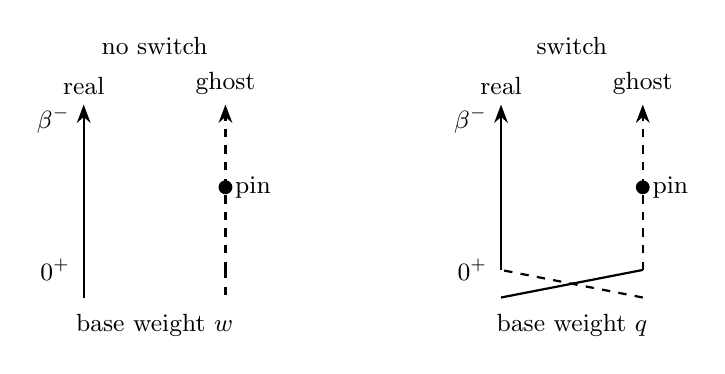
\begin{tikzpicture}[x=1cm,y=1cm,>=Stealth,font=\small]
 \foreach \x/\lab in {0/{no switch},5.3/{switch}} {
  \node at (\x+1.3,3.25) {\lab};
  \draw[->,thick] (\x+.4,.4)--(\x+.4,2.5);
  \draw[->,thick,dashed] (\x+2.2,.4)--(\x+2.2,2.5);
  \node[above] at (\x+.4,2.5) {real};
  \node[above] at (\x+2.2,2.5) {ghost};
  \fill (\x+2.2,1.45) circle (2.5pt);
  \node[right] at (\x+2.2,1.45) {pin};
  \node[left] at (\x+.35,.4) {\(0^+\)};
  \node[left] at (\x+.35,2.3) {\(\beta^-\)};
 }
 \draw[thick] (.4,.4)--(.4,.05);
 \draw[thick,dashed] (2.2,.4)--(2.2,.05);
 \node at (1.3,-.3) {base weight \(w\)};
 \draw[thick] (5.7,.05)--(7.5,.4);
 \draw[thick,dashed] (7.5,.05)--(5.7,.4);
 \node at (6.6,-.3) {base weight \(q\)};
\end{tikzpicture}

 \caption{One real slot and its stationary ghost, shown on a cut-open
 time circle.  An absent switch leaves the ghost as a separate pinned
 cycle.  A present switch inserts its pinned line into the real cycle.
 In the unconditioned fresh real-hole traversal killed on entry into a ghost, passage through
 this layer survives with probability \(w=1-q\).  The rest of the
 real exchange picture is suppressed.}
 \label{fig:sparse-ghost}
\end{figure}

Let \(E\) denote all the ghost pins together with any finite set of
deterministic real-slot pins.  We write \(\PP_E\) for the normalized
picture law with density proportional to \(2^{c_E}\), and
\(\mathcal B_E\) for the slot-time points on cycles missing \(E\).
These cycles contain only real slots.  At coincident prescribed
operations, a slot point means the point just after the entire ordered
bundle, as in Section~\ref{sec:exchange}.  Distances
between sites are wrapped supremum distances, denoted \(d_L\); balls
are denoted by \(B_h(z)\).

Fix \(\alpha=1/100\) and a sufficiently large constant \(C_s\ge6\).
A finite collection of real slot points is \emph{sparse} if its site
coordinates, counted with multiplicity, satisfy
\begin{equation}\label{eq:torus-sparse}
 \#\{i:x_i\in B_h(z)\}\le C_s(1+h)^\alpha
 \qquad(z\in\Lambda_L,\ h\ge0).
\end{equation}
The same definition applies to lists of centers.  In particular,
different slots at the same site count separately.  The freedom to
choose \(C_s\) large will permit the finite collections of nearby
test points used in Section~\ref{sec:spatial-comparison}.

\begin{proposition}[Sparse-pin bound]\label{prop:sparse-pins}
Fix \(S\) and \(C_s\).  There is \(\beta_0<\infty\) such that, for
every fixed \(\beta\ge\beta_0\), there is \(L_*(\beta)<\infty\)
with the following property.  For every even \(L\ge L_*(\beta)\),
every \(q\) satisfying \(L^{-5/2}\le q<1\), every pin set \(E\)
as above, and every sparse set \(T\) of real slot points at one
deterministic time,
\begin{equation}\label{eq:sparse-pins}
 \PP_E(T\subseteq\mathcal B_E)\le p^{|T|},
 \qquad p=\beta^{-9/10}.
\end{equation}
The constants and thresholds are independent of the number, locations,
and times of the extra pins.
\end{proposition}

The proof is a finite downward induction on deterministic pins.
Its larger-pin hypothesis gives regular hole graphs; diffusion and a
flow-energy estimate then make next-pin returns rare enough to remove
the test pins by Lemma~\ref{lem:pin-inputs}.

If \(T\) is empty the assertion is immediate; if it meets \(E\),
the event is impossible.  We henceforth consider nonempty
\(T\cap E=\varnothing\), put \(P=E\cup T\), and expose the cycles
missing \(P\) under \(\PP_P\).  All other slot points are called
\emph{holes}.  Lemmas~\ref{lem:pin-inputs} and~\ref{lem:next-pin}
apply to this enlarged picture.  Here are the details concerning ghosts.

For any proposed set of exposed time-zero real labels, reveal its
trajectories, its seam images, and the switch outcomes encountered by
those trajectories.  Closure into cycles avoiding \(P\) requires every
such switch to be absent.  Separate Poisson clocks according to whether
they touch the currently exposed labels, as in the exposure
disintegration of Lemma~\ref{lem:pin-inputs}.  Conditional on the
revealed histories, the unused clocks are fresh on pairs of holes;
the remaining seam images are uniform completions within each site;
and switches on the other real--ghost pairs are still independent
Bernoulli switches.  When an exposed label jumps through a hole, that
hole is transported in the opposite direction.  A mark between two
exposed labels does not move a hole.  Requiring these to be all the
missing cycles conditions the fresh picture on every remaining cycle
meeting \(P\).  The exposed cycles contribute only their fixed factor
\(2^{c_P}\); therefore this description gives the conditional law,
including its all-hit conditioning.  That conditioning has positive
probability at almost every exposure.

Every ghost is a hole and is pinned.  Missing real cycles never use a
switch, so the number of real holes is constant in time.  The seam
does not change their number at any site.  In particular the
factorial-mark estimate in Lemma~\ref{lem:pin-inputs} remains valid:
inserting a real-edge transposition changes the number of missing
cycles by at most one, even in the presence of switches.

By Lemma~\ref{lem:next-pin}, conditional next-pin probabilities are
first-hit probabilities for the unconditioned fresh walk, with fresh
transitions on each repeated traversal.  Delete the other real-pin
stops and kill that walk on entering a ghost.  This only increases the
probability that its next pin belongs to \(T\): after entering a ghost,
the walk encounters its pin before its next opportunity to return to a
real slot.  The one-turn real-hole kernel at the time of \(T\) is
\begin{equation}\label{eq:ghost-mass}
 U=wK,\qquad U_+=U,\quad U_-=U^*,\quad Q=\tfrac12(U+U^*),
 \qquad E_y=\ip{y}{(I-Q)y}\ge q\norm{y}_2^2.
\end{equation}
Here and throughout this section matrices are column-forward.
The matrix \(K\) is doubly stochastic: its factors are symmetric
hole-walk heat kernels, forced transport bijections, and uniform
remaining seam completions.  Exactly one switch layer is crossed per
turn, and its real-to-real mean is \(wI\), which proves \(U=wK\).
All factors, their adjoints, and spatially killed versions contract
counting \(1\)-, \(2\)-, and supremum norms.  For example, a
nonnegative matrix whose row and column sums are at most one satisfies
\(\sum_i|(Av)_i|^2\le\sum_{i,j}A_{ij}|v_j|^2\le\norm v_2^2\).
This also proves the last inequality in \eqref{eq:ghost-mass}.

\subsection{The deterministic geometric input}

We state precisely the infinite-lattice results that will be transferred
to the torus.  An available-slot graph on \(\Z^3\) has between zero
and \(\ell\) slots at each site, all \(\ell\) slots outside a finite
set, and all pairs of available slots joined across every
nearest-neighbor site bond.  A site with no available slot is
\emph{blocked}.  Join blocked sites at supremum distance at most eight
and write \(\mathcal C(w)\) for the component of a blocked site \(w\).
Fix \(\nu=1/300\).  The constants \(M_*\) and \(A_0\) below depend
only on this lattice geometry and \(\ell\).

A graph is \emph{regular at \(z\) with radius \(A\ge A_0\)} if
\begin{enumerate}[label=(\roman*)]
 \item every ball \(B_{M_*}(v)\), with \(v\in B_{11A}(z)\),
 contains fewer than six blocked sites;
 \item each blocked \(w\notin B_{10A}(z)\) satisfies
 \(\max_{v\in\mathcal C(w)}|v-w|_\infty
       \le(1+|w-z|_\infty)^\nu\).
\end{enumerate}
The anchor itself need not have an available slot.
One may take \(M_*\ge\max\{48,\rho(3,44)+2\}\), where the
local-connectivity radius \(\rho(3,44)\) has the following property:
two unblocked sites at distance at most 44 can be joined inside
\(B_{\rho(3,44)}\) about the first site if that ball contains fewer
than six blocked sites.  The path has length at most
\((2\rho(3,44)+1)^3\).  This is
\cite[Lemma~5.5 and Equation~(5.13)]{Ord}; regularity is
\cite[Definition~3.2]{BL}, equivalently
\cite[Definition~5.3]{Ord}.  Take \(A_0\ge M_*+47\) large enough
for the following two conclusions.

\begin{lemma}[Lattice Nash inequality and unit flows]\label{lem:lattice-inputs}
In an available-slot graph regular at \(z\) with radius \(A\ge A_0\),
put
\[
 \mathcal D(v)=\tfrac12\sum_{\{i,j\}\text{ available edge}}
                              (v_i-v_j)^2.
\]
Every nonnegative \(v\) supported over \(B_A(z)\) satisfies
\begin{equation}\label{eq:local-nash}
 \norm v_2^{10/3}\le C\mathcal D(v)\norm v_1^{4/3}.
\end{equation}
For every available slot \(a\) at \(y\in B_A(z)\), there exists
an oriented edge flow \(F_a\), with divergence defined as outgoing
minus incoming flow, such that
\begin{equation}\label{eq:unit-flow}
 \Div F_a=\1_{\{a\}},\qquad
 |F_a(e)|\le C(1+\dist(e,y))^{-k},\qquad
 k=2-3\nu=199/100.
\end{equation}
Here \(\dist(e,y)\) is the minimum supremum distance to the two
endpoint sites.  The constants are uniform over the graph, \(A\),
\(z\), and the source.  Sites with any number of available slots
between one and \(\ell\) are permitted.
\end{lemma}

These are \cite[Proposition~3.3 and Lemma~3.4]{BL}; the underlying
geometric constructions are \cite[Propositions~5.6 and~6.2]{Ord}.
Their hypotheses are deterministic and impose no relation between
\(A\) and a time scale.  Only these stated conclusions of the
infinite-lattice results will be used here.

At a given exposure and physical time, make such a graph for each
torus anchor \(z\): lift the real holes in \(B_{\lfloor L/4\rfloor}(z)\)
to \(\Z^3\), and declare every slot outside this box available.
We say the slice is regular at \(z\) when this graph is regular.
We shall use
\begin{equation}\label{eq:sparse-localization-radius}
 A=\lceil C_{\mathrm{loc}}\beta\rceil,
 \qquad 11A+M_*<\lfloor L/4\rfloor,
\end{equation}
where \(C_{\mathrm{loc}}\) is fixed sufficiently large below.
Thus the Nash inequality for functions supported in \(B_A(z)\)
uses exactly the torus edges, with zero values beyond the support.

\subsection{From grid pins to regular slices}

Choose a finite circular grid \(\mathcal G\) containing zero, with
successive gaps at most \(p^{12}\).  For a set \(P\) of ghost pins
and real pins on this grid, let \(\mathsf I(P)\) assert
\eqref{eq:sparse-pins} under \(\PP_P\) for every sparse test at
one grid time.  In this subsection we assume \(\mathsf I(P)\).
This is the hypothesis for a larger pin set in the eventual downward
induction; no estimate for a smaller pin set is assumed.

At time \(t\), write \(\mathcal O_t\) for the sites without a real
hole.  At a grid time, simultaneous blocking of prescribed sparse
sites costs at most \(p^n\): choose one fixed slot at each site and
apply \(\mathsf I(P)\).  If any chosen slot is pinned, the event is
impossible.  The same conclusion can therefore be used without
checking disjointness separately.

\begin{lemma}[Blocking and component tails]\label{lem:torus-blocking}
Under \(\mathsf I(P)\), at any deterministic time \(t\),
\begin{align}
 \PP_P(A'\subseteq\mathcal O_t)&\le Cp^6
 &&\text{for six prescribed distinct sites},\label{eq:six-blocking}\\
 \PP_P(A'\subseteq\mathcal O_t)&\le(C\sqrt p)^{|A'|}
 &&\text{for a nonempty sparse set of sites}.\label{eq:sparse-blocking}
\end{align}
There are \(c,C,\lambda>0\), uniform for sufficiently large \(\beta\),
such that the blocked component formed with steps of supremum length
at most eight satisfies
\begin{equation}\label{eq:torus-component-tail}
 \PP_P\{z\in\mathcal O_t,\ 
       \max_{v\in\mathcal C_t(z)}d_L(z,v)\ge h\}
       \le C e^{-ch^\lambda}\qquad(h\ge1).
\end{equation}
All constants are independent of the grid and its size.
\end{lemma}

\begin{proof}
Let \(s\) be the grid point preceding \(t\), with \(s=t\) if
\(t\in\mathcal G\).  A site blocked at \(t\) either was blocked at
\(s\), or has an incident real-edge mark in \((s,t]\).  The seam
preserves hole counts at each site; the switch layer also preserves
the real-hole set of an exposure, as observed above.  The union of
the stars of six sites has bounded total intensity.  Factorial
domination in Lemma~\ref{lem:pin-inputs} bounds the probability of a
mark there by \(Cp^{12}\), giving \(p^6+Cp^{12}\le Cp^6\).

For \(n\) sparse sites, either at least \(\lceil n/2\rceil\)
were blocked at \(s\), costing at most
\(2^np^{\lceil n/2\rceil}\), or at least that many have incident
marks.  A mark touches at most two of the selected sites, so the
second alternative requires \(j=\lceil n/4\rceil\) distinct marks.
The union of the stars has intensity at most \(Cn\); hence its
probability is at most
\[
 \frac{(Cnp^{12})^j}{j!}\le(C'p^{12})^j,
\]
using \(j!\ge(j/e)^j\) and \(n/j\le4\).  Enlarging the constant
gives \eqref{eq:sparse-blocking}, without an independence assumption
between the two alternatives.

For the component tail, fix an integer \(a>100\) so large that
\(a^\alpha>4\), and set \(h_j=16a^j\).  A blocked path from
\(z\) to wrapped distance \(h_j\) yields two smaller crossings:
the first starts at \(z\), and the second at the first path site at
distance at least \(h_j/2\) from \(z\).  Truncate each at its
first reach of distance \(h_{j-1}\) from its own start.  The starts
are between \(h_j/2\) and \(h_j/2+8\) apart, and each truncated
crossing stays within radius \(h_{j-1}+8\).  Thus their mutual
distance is at least
\(h_j/2-2(h_{j-1}+8)\ge h_j/4\).  The remaining portion of the
original crossing has sufficient length for the second truncation,
since its endpoint is at least \(h_j/2-8\) from the second start.
These statements use only the triangle inequality for wrapped distance.

Recursion gives an ordered binary witness with \(2^j\) distinct
blocked leaves.  At every split of scale \(h_k\) the two descendant
leaf sets are at distance at least \(h_k/4\).  Therefore a ball of
radius less than \(h_k/8\) meets at most one branch at each split
of scale \(h_k\) or larger, and contains at most \(2^{k-1}\)
leaves.  For \(h_{k-1}/8\le h<h_k/8\), this is bounded by
\(C_s(1+h)^\alpha\), because \(a^\alpha>4\).  Below \(h_0/8\)
there is at most one leaf, and at or above \(h_j/8\) the same
comparison allows all \(2^j\) leaves.  Hence every such witness
is sparse, at every center and every radius.

At a split of scale \(h_k\), the second start has at most
\(Ch_k^3\) choices on the torus.  If \(W_j\) bounds the number
of witnesses rooted at a prescribed site, then
\[
 W_0=1,\quad W_j\le Ch_j^3W_{j-1}^2,\quad
 2^{-j}\log W_j\le\sum_{k\ge1}2^{-k}\log(Ch_k^3)<\infty.
\]
Thus \(W_j\le C_a^{2^j}\).  This count may ignore separation,
but the probability bound is applied only to the separated witnesses
just constructed.  Equation~\eqref{eq:sparse-blocking} bounds their
union by \((C_aC\sqrt p)^{2^j}\), which is at most
\(e^{-2\cdot2^j}\) for sufficiently large \(\beta\).
For \(h_j\le h<h_{j+1}\), use \(\lambda=\log_a2\) and
\(2^j\ge(h/(16a))^\lambda\).  Bounded \(h\) is absorbed by
\(C\); if \(h\) exceeds the torus diameter the event is empty.
This proves \eqref{eq:torus-component-tail}.
\end{proof}

\begin{lemma}[Regularity and localized diffusion]\label{lem:torus-diffusion}
Assume \(\mathsf I(P)\) and \eqref{eq:sparse-localization-radius}.
For every deterministic time and anchor, failure of regularity has
probability at most
\begin{equation}\label{eq:torus-irregularity}
 \Delta_A=CA^3p^6+C\exp(-cA^{\lambda\nu}).
\end{equation}
Call an exposure good at the anchor if its nonregular times have total
length at most \(\beta/100\).  Its probability of not being good is
at most \(100\Delta_A\).  On a good exposure, the one-turn kernel
localized by killing outside \(B_A(z)\) has every entry at most
\(C\beta^{-3/2}\), in either direction.

If a deterministic starting slot is a hole almost surely, localization
at its site loses at most \(Ce^{-c\beta}\) expected mass in any
forward or reversed traversal piece of length at most one turn.  This
last assertion does not require \(\mathsf I(P)\).
\end{lemma}

\begin{proof}
There are \(O(A^3)\) centers in \(B_{11A}(z)\), and a fixed
\(M_*\)-ball has only a bounded number of six-site subsets.
Equation~\eqref{eq:six-blocking} therefore gives \(CA^3p^6\)
for failure of local regularity.  For a remote blocked site at lifted
distance \(r>10A\), failure of the other condition costs at most
\(C\exp[-c(1+r)^{\lambda\nu}]\), by
\eqref{eq:torus-component-tail}.  Indeed all blocked sites of the
lift lie in its radius-\(\lfloor L/4\rfloor\) box, so coordinate
differences between them are at most \(L/2\) and equal their wrapped
distances.  A crossing in a lifted component is a crossing in the
torus component.  Summing the remote bound over shells, each containing
at most \(C(1+r)^2\) sites, gives the second term of
\eqref{eq:torus-irregularity}, with a smaller exponential rate.
Fubini and Markov give the asserted probability for a good exposure.

Let \(v(u)\) be a localized evolving nonnegative mass, initially of
mass at most one, and put \(H(u)=\norm{v(u)}_2^2\).  On smooth intervals,
with zero extension across the killing boundary,
\[
 H'=-2\mathcal D_t(v).
\]
The energy is the sum of \(\tfrac12(v_i-v_j)^2\) over unordered
real-hole edges, including edges from surviving to killed positions.
At a regular time, Lemma~\ref{lem:lattice-inputs} gives
\(H'\le-cH^{5/3}\).  At other times and at instantaneous
factors, the squared norm cannot increase.  Unless it has become zero,
\((H^{-2/3})'\ge c'\) throughout the regular times.
Each half turn has at least \(\beta/2-\beta/100\) regular time,
so its output has \(2\)-norm at most \(C\beta^{-3/4}\).
The same proof applies to its adjoint, since heat factors are
symmetric, transports reverse by bijections, and seam completions
reverse by uniform inverse completions.  Split a full turn at its
temporal midpoint and apply Cauchy--Schwarz to the two resulting
masses.  This proves the entry bound.

For localization, sample the complete picture under \(\PP_P\),
and independently supply fresh Poisson clocks for the hole walk,
accepted where both endpoints are holes.  Forced transports use
actual picture marks; seam and switch operations do not change sites.
An exit from \(B_A(z)\) needs at least \(A\) inter-site steps.
In a traversal piece of length at most \(\beta\), the physical
times run injectively through at most one period, whether forward,
backward, or across the seam.  Thus the actual marks used by these
steps are distinct, as are the fresh marks.  Ignore slot compatibility
and count site paths.  There are boundedly many choices of the next
site, slot edge, and actual-or-fresh clock at each step.  The factorial
bound of Lemma~\ref{lem:pin-inputs}, combined with the independent
fresh factorial measure, bounds the expected number of ordered lists
of \(j\) steps from the starting site by
\[
 \frac{(C\beta)^j}{j!}.
\]
The denominator is the volume factor for the ordered time simplex.
Taking \(j=A\) and \(C_{\mathrm{loc}}\) sufficiently large makes
this at most \(Ce^{-c\beta}\), using \(j!\ge(j/e)^j\).
This is an unconditional estimate under the correct exposure marginal;
no fresh-clock estimate under the all-hit conditioning is needed.
\end{proof}

\subsection{Cutting off the flows}

Localized diffusion controls a direct one-turn return.  A return after
many turns will instead be controlled by an energy inequality.  The
following finite-torus form of the sparse-source estimate isolates the
only error introduced by replacing a pinned boundary with ghost killing.

\begin{lemma}[Sparse-source pairing on the torus]\label{lem:torus-flow-pairing}
At a fixed slice let \((z_i)_{i=1}^{m_T}\) be a sparse list, including
repetitions.  Retain any subset of its members at which the lifted
graph is regular with radius \(A\).  For each retained member let
\(\mu_i\ge0\) be a mass at most one, supported on the real holes
over \(B_A(z_i)\).  If \(L\) satisfies
\eqref{eq:sparse-localization-radius} and is sufficiently large
compared with \(A\), then every real vector \(Y'\) on the holes
of that slice satisfies
\begin{equation}\label{eq:torus-flow-pairing}
 \left|\left\langle\sum_i\mu_i,Y'\right\rangle\right|
 \le (Cm_TA^\alpha)^{1/2}\sqrt{\mathcal D_t(Y')}
      +Cm_TL^{1/2-k}\norm{Y'}_2.
\end{equation}
\end{lemma}

\begin{proof}
For an individual source slot \(a\) in the support of \(\mu_i\),
take the flow of Lemma~\ref{lem:lattice-inputs} in the lift about
\(z_i\).  Multiply its value on each edge by a taper equal to one
within anchor radius \(L/10\), zero beyond radius \(L/5\), and
with Lipschitz constant \(C/L\).  For instance use a piecewise linear
function of the supremum distance of the edge midpoint.  The support
is strictly inside the lifted box, so this cut flow projects to a flow
\(\widetilde F_a\) on the torus real-hole graph.

Its divergence has the form \(\1_{\{a\}}+\varepsilon_a\).
To see the error bound, compare the taper at an incident edge with
its value at the vertex.  Their difference is at most \(C/L\);
the untapered divergence is zero except at \(a\), where the taper
is one.  In the transition annulus every edge is at distance comparable
with \(L\) from the source, because \(A\ll L\).  The bounded
degree and \eqref{eq:unit-flow} give
\[
 |\varepsilon_a(j)|\le CL^{-k-1},\qquad
 \norm{\varepsilon_a}_2\le CL^{1/2-k}.
\]
No discrepancy arises outside that annulus enlarged by one lattice
step, and there are at most
\(CL^3\) slots in it.

The projected flow retains the bound
\(C(1+d_L(e,x_a))^{-k}\).  For two source sites at wrapped
distance \(h\), the sum of the product of these envelopes is at most
\begin{equation}\label{eq:torus-flow-overlap}
 C(1+h)^{-(2k-3)}.
\end{equation}
For \(h\ge3\), inside the radius-\(h/3\) ball about either source,
one envelope is at most \(Ch^{-k}\) and the sum of the other is at
most \(Ch^{3-k}\).  Outside both balls, dyadic shells of radii at
least \(h/3\) contribute at most
\(C\sum_{r\ge0}(2^rh)^{3-2k}\).  Shell counts on the torus are
bounded by the corresponding lattice counts.  Since \(2k>3\),
this proves \eqref{eq:torus-flow-overlap}; bounded \(h\) follows
from square summability of the envelopes.

Sum the cut flows with the source masses as coefficients and denote
the result by \(F\).  For centers at distance at most \(4A\),
use the constant overlap bound; for more distant centers, every pair
of their source sites is at least half as far apart.  With
\(\sigma=2k-3=49/50>\alpha\), sparseness and dyadic annuli give
\begin{align*}
 \norm F_2^2
 &\le C\sum_i\left(\#\{j:d_L(z_i,z_j)\le4A\}
       +\sum_{j:d_L(z_i,z_j)>4A}(1+d_L(z_i,z_j))^{-\sigma}\right)\\
 &\le Cm_T\left(A^\alpha+
          \sum_{r\ge0}(2^rA)^{\alpha-\sigma}\right)
 \le Cm_TA^\alpha.
\end{align*}
This calculation uses only that each mass is at most one; it permits
both overlapping supports and repeated centers.  The summed divergence
error \(\varepsilon\) has
\(\norm\varepsilon_2\le Cm_TL^{1/2-k}\).  Finally,
\[
 \left\langle\sum_i\mu_i,Y'\right\rangle
 =\sum_eF(e)(Y'_{e^-}-Y'_{e^+})-\ip{\varepsilon}{Y'}.
\]
Cauchy--Schwarz, with
\(\sum_e(Y'_{e^-}-Y'_{e^+})^2=2\mathcal D_t(Y')\), proves the
claim.  The empty retained subset gives zero and is included.
\end{proof}

\subsection{Return energy and completion of the induction}

We now prove Proposition~\ref{prop:sparse-pins}.  Fix a grid and
argue by downward induction over its finite set of real slot points.
When every such point is pinned, \(\mathsf I(E)\) is immediate.
Assume the assertion for every strict superset of \(E\), and choose
a nonempty sparse grid test \(T\) disjoint from \(E\).  Then
\(P=E\cup T\) satisfies \(\mathsf I(P)\), so all the preceding
blocking and diffusion estimates hold under \(\PP_P\).

At an exposure under that law put \(m_T=|T|\) and
\(\zeta=\1_T\).  Let \(F=1\) on \(T\), and elsewhere let
\(F\) be the probability that the ghost-killed walk with kernel
\(U\) ever hits \(T\) at a later cut.  Explicitly, start with
\(F_0=\zeta\) and iterate
\(F_{n+1}=1\) on \(T\), \(F_{n+1}=U^*F_n\) off \(T\).
These vectors increase to \(F\), with \(0\le F\le1\) and
\(U^*F=F\) off \(T\).  Set \(g=F-\zeta\), so
\(0\le g\le1\) and \(g=0\) on \(T\).

Let \(r(E,T)\) be the mean, over \(\PP_P\) and the uniform
starting point in \(T\), of the indicator that its next pin is
in \(T\).  The pin inequality of Lemma~\ref{lem:pin-inputs} is
\begin{equation}\label{eq:sparse-pin-reduction}
 \PP_E(T\subseteq\mathcal B_E)\le(2r(E,T))^{m_T}.
\end{equation}
Conditionally on the exposure, deletion of the other real-pin stops
bounds the sum of these next-pin probabilities by
\(\sum_{i\in T}(U^*F)_i\).  Harmonicity off \(T\) gives
\begin{align}
 \sum_{i\in T}(U^*F)_i
 &=m_T-\ip F{(I-Q)F}\notag\\
 &=\ip\zeta{Q\zeta}+2\ip{Q\zeta}g-E_g.
 \label{eq:torus-hitting-energy}
\end{align}
Indeed the quadratic forms of \(U,U^*,Q\) agree on real vectors,
and \(\ip\zeta g=0\).  In particular no reversibility of \(U\)
has been assumed.

The first term is controlled by one-turn diffusion.  Start a unit mass
at each \(i\in T\) and localize at its site, in either direction.
Lemma~\ref{lem:torus-diffusion} bounds discarded mass in expectation
by \(Ce^{-c\beta}\).  On a good exposure there are at most
\(C_s(1+A)^\alpha\) target points of \(T\) in its localized
region, each receiving at most \(C\beta^{-3/2}\).  A nongood
exposure has probability at most \(100\Delta_A\) and still carries
total mass at most one.  Thus
\begin{equation}\label{eq:torus-short-return}
 \E_P\ip\zeta{Q\zeta}
 \le Cm_T\bigl(e^{-c\beta}+\Delta_A+A^\alpha\beta^{-3/2}\bigr).
\end{equation}

To absorb the linear term in \eqref{eq:torus-hitting-energy}, split
the traversal in direction \(d\in\{+,-\}\) at elapsed time
\(u\in I=[\beta/3,2\beta/3]\):
\[
 U_d=B_d(u)C_d(u),\qquad Y_d(u)=B_d(u)^*g.
\]
The factors use matching hole layers at physical time
\(t_d(u)=\theta+u\) or \(\theta-u\) modulo \(\beta\), where
\(\theta\) is the cut of \(T\).  Each instantaneous factor is
assigned to exactly one side; the finitely many exceptional split
times do not affect the integrals.  As \(u\) decreases, \(Y_d(u)\)
accumulates adjoint factors from the endpoint.  Its continuous norm
loss is twice its Dirichlet energy, and instantaneous factors contract.
Consequently
\begin{equation}\label{eq:torus-suffix-energy}
 \int_I\mathcal D_{t_d(u)}(Y_d(u))\dd u
 \le\tfrac12\bigl(\norm g_2^2-\norm{U_d^*g}_2^2\bigr)
 \le E_g.
\end{equation}
The second inequality follows from the exact identity
\[
 E_g-\tfrac12(\norm g_2^2-\norm{U_d^*g}_2^2)
       =\tfrac12\norm{g-U_d^*g}_2^2,
\]
because \(\ip g{U_d^*g}=\ip g{Qg}\).
Also \(\norm{Y_d(u)}_\infty\le1\) and
\(\norm{Y_d(u)}_2\le\norm g_2\).

For each \(i\in T\), propagate its unit mass by the starting
portion \(C_d(u)\), with localization at \(z_i=x_i\), and retain
it only when the slice is regular at \(z_i\).  Call the resulting
sum \(M_d(u)\), and put
\[
 J_d=|I|^{-1}\int_I\ip{M_d(u)}{Y_d(u)}\dd u.
\]
The original pairing
\(\ip{C_d(u)\zeta}{Y_d(u)}=\ip{U_d\zeta}g\) is constant in
\(u\).  Supremum contraction, localization, and the deterministic-time
bound \eqref{eq:torus-irregularity} show that
\begin{equation}\label{eq:torus-pairing-error}
 \E_P\left|\ip{U_d\zeta}g-J_d\right|
 \le Cm_T(e^{-c\beta}+\Delta_A).
\end{equation}
This uses Fubini and only regularity at the split, without requiring a
good exposure over the entire turn.

Apply Lemma~\ref{lem:torus-flow-pairing} to the retained masses.
Cauchy--Schwarz in \(u\), \eqref{eq:torus-suffix-energy}, and
\(E_g\ge q\norm g_2^2\) give the pointwise bound
\begin{equation}\label{eq:torus-linear-energy}
 |J_d|\le C\left((m_TA^\alpha/\beta)^{1/2}
           +m_TL^{1/2-k}/\sqrt q\right)\sqrt{E_g}.
\end{equation}
Since \(2\ip{Q\zeta}g=\ip{U_+\zeta}g+\ip{U_-\zeta}g\),
we complete the square in \(\sqrt{E_g}\) to obtain
\[
 J_++J_--E_g
 \le C\left(m_TA^\alpha/\beta+m_T^2L^{1-2k}/q\right).
\]
Combining this with \eqref{eq:torus-short-return} and
\eqref{eq:torus-pairing-error}, and dividing by \(m_T\), yields
\begin{equation}\label{eq:torus-return-bound}
 r(E,T)\le C\left(e^{-c\beta}+\Delta_A
     +A^\alpha\beta^{-3/2}+A^\alpha/\beta
     +m_TL^{1-2k}/q\right).
\end{equation}

Every constant so far is independent of the grid, its number of
points, and the induction pin set.  Sparseness gives
\(m_T\le C L^\alpha\); because \(q\ge L^{-5/2}\), the last term
of \eqref{eq:torus-return-bound} is at most
\[
 C L^{\alpha+7/2-2k}=C L^{-47/100}.
\]
The remaining terms, with \(A=\lceil C_{\mathrm{loc}}\beta\rceil\),
are \(o(p)\) as \(\beta\to\infty\): their polynomial orders are
\(\beta^{-12/5}\), \(\beta^{-149/100}\), and
\(\beta^{-99/100}\), besides stretched-exponential terms.
Choose \(\beta_0\) sufficiently large first.  For each fixed
\(\beta\ge\beta_0\), choose \(L_*(\beta)\) sufficiently large
for \eqref{eq:sparse-localization-radius} and for the last term to
make \(2r(E,T)\le p\).  Equation~\eqref{eq:sparse-pin-reduction}
then proves \(\mathsf I(E)\), completing the finite induction.

For arbitrary finite extra pins and a test at any deterministic time,
choose a grid containing their times and zero, and refine it to mesh
at most \(p^{12}\).  Uniformity in the grid gives the proposition
without a limiting procedure.  In particular the blocking,
component-tail, and regularity conclusions above now hold under every
allowed pin law.  All time integrals are measurable: the finite-volume
histories have finitely many jumps, their kernels are products of
measurable heat and instantaneous matrices, and the hitting function
is an increasing limit of finite-horizon probabilities.  No choice of
the auxiliary flows has to be measurable, since only their deterministic
pairing inequality is used.

\begin{corollary}[Positive spontaneous magnetization]\label{cor:positive-magnetization}
For every fixed \(S\) and all sufficiently large finite \(\beta\),
\[
 m_{S,\beta}\ge S(1-\beta^{-9/10})>0.
\]
\end{corollary}

\begin{proof}
The passage from pinned-cycle probabilities to the pressure slope uses
pressure increments, as in \cite[Section~7]{BL}.  Fix \(\beta\)
above the threshold of Proposition~\ref{prop:sparse-pins}, enlarged
so that \(\beta>1\), and put \(p=\beta^{-9/10}\).  For an exponent
field \(s>0\), set \(q(s)=1-e^{-s}\), and use the ghost picture
with no extra real pins.  A real slot is down with probability one
half of its probability of belonging to a cycle missing the ghost
pins: pinned cycles are up, and missing cycles are colored fairly.
The singleton case of Proposition~\ref{prop:sparse-pins} therefore
gives a down probability at most \(p/2\), whenever
\(L\ge L_*(\beta)\) and \(q(s)\ge L^{-5/2}\).

Define the finite-volume exponent pressure
\[
 \mathcal P_L(s)=V^{-1}\log\Tr
       \exp\!\left(H_0+s\sum_xY_x\right).
\]
Write \(\langle\cdot\rangle_s\) for the corresponding tilted Gibbs
expectation.
There are \(\ell V\) slots and \(\ell=2S\), so differentiation
and the color representation give
\[
 \mathcal P_L'(s)
   =V^{-1}\left\langle\sum_xY_x\right\rangle_s
   \ge S(1-p).
\]
For fixed \(0<a<b\), this holds simultaneously for all
\(s\in[a,b]\) once
\(L\ge\max\{L_*(\beta),q(a)^{-2/5}\}\).  Integration yields
\[
 \mathcal P_L(b)-\mathcal P_L(a)\ge S(1-p)(b-a).
\]
By rotation invariance and the pressure limit \eqref{eq:pressure},
\(\mathcal P_L(s)\to\mathcal P(s)=\beta p_{S,\beta}(s/\beta)\)
along even \(L\).  Pass to this limit first.  The limiting pressure
is \(S\)-Lipschitz, because
\(\norm{\sum_xY_x}\le SV\); letting \(a\downarrow0\) therefore
gives \(\mathcal P(b)-\mathcal P(0)\ge S(1-p)b\).
Finally divide by \(b\) and let \(b\downarrow0\).  Since
\(\mathcal P'(0+)=p_{S,\beta}'(0+)=m_{S,\beta}\), this proves
the claim with the volume limit taken before removal of the field.
\end{proof}

\section{Spatial comparison at a vanishing field}\label{sec:weak-field}
\label{sec:spatial-comparison}

The sparse-pin estimate controls the missing cycles at prescribed
points.  We now turn it into a bound for a spatially oscillating
magnetization.  The two steps are quite different.  First, an exact
susceptibility identity expresses the transverse square through a
one-particle resolvent on the holes.  Second, we show that the resolvent
is nearly constant on large rectangular cells.  Small closed classes of
holes are allowed; a trace identity controls their total contribution.

\begin{proposition}[Weak-field spatial estimate]\label{prop:weak-field}
Fix $S$.  For all sufficiently large $\beta$ there are
$C_\beta,R_0(\beta)<\infty$ with the following property.  Let $L$ be
even, let $R_0(\beta)\le R\le L$, and partition $\Lambda_L$ into
rectangular cells whose side lengths belong to $[R/2,4R]$.  For every
deterministic real $f:\Lambda_L\to[-1,1]$ with
$\sum_{x\in B}f_x=0$ on each cell $B$, put
\[
 D_f=\sum_x f_x Z_x,\qquad q=R^{-5/2},\qquad
 w=1-q=e^{-b}.
\]
If $\langle\cdot\rangle_b$ is the Gibbs expectation with exponent
$H_0+b\sum_xY_x$, then
\begin{equation}\label{eq:weak-field}
 \frac qV\langle D_f^2\rangle_b\le C_\beta R^{-1/40}.
\end{equation}
The constants are uniform in the partition, $f$, and $L$.
\end{proposition}

Throughout the proof $\beta$ is fixed above a sufficiently large
threshold; subsequent lower bounds on $R$ may depend on $\beta$.
We use the soft-pin representation of Section~\ref{sec:sparse-pins},
with no extra deterministic real pins.  Expose all cycles missing the
soft pins.  Write $\mathbf a$ for their trajectories, $A_0$ for their
real slots at the cut, and $\mathcal H$ for the complementary cut
slots, called the holes.  The cut is after the seam and its soft-pin
insertions, which do not move any line.
The soft pins themselves may be placed on real cut slots, instead of
using the equivalent ghosts.  A hole cycle is then pinned and has up
color; every exposed cycle receives an independent fair color.

\subsection{The susceptibility as a hole resolvent}

Condition on $\mathbf a$.  The fresh real-hole motion consists of
rate-$1/2$ jumps across the currently available slot edges, the forced
hole transports at exposed jumps, and a uniform completion of the seam
permutation within each site.  Its one-turn kernel, without killing
or conditioning on its cycles, is denoted by $K$.  In this section we
use the \emph{row-forward convention}: $K_{ij}$ is the probability
of going from $i$ to $j$.  Thus $K$ is doubly stochastic.  Set
\begin{equation}\label{eq:hole-resolvent}
 D=I-wK,\qquad D^{-1}=\sum_{r\ge0}w^rK^r.
\end{equation}
This inverse exists and is entrywise nonnegative.  Empty hole sets use
empty matrices, determinant one, and sums zero.

\begin{lemma}[Soft-pin identities]\label{lem:soft-resolvent}
Given the exposure $\mathbf a$, for $i,j\in\mathcal H$, $i\ne j$,
\begin{align}
 \PP(i\text{ is pinned}\mid\mathbf a)
   &=q(D^{-1})_{ii},\label{eq:pin-marginal}\\
 \PP(i,j\text{ are pinned, next pin from }i\text{ is }j
            \mid\mathbf a)
   &=\frac{q^2}{w}(D^{-1})_{ij}.\label{eq:pin-successor}
\end{align}
Moreover,
\begin{equation}\label{eq:resolvent-trace}
 \E\Tr D^{-1}\le N.
\end{equation}
For $f_i=f_{x_i}$ on the slots,
\begin{equation}\label{eq:transverse-resolvent}
 \langle D_f^2\rangle_b
 =\frac14\sum_i f_i^2+
   \frac12\E\sum_{\substack{i,j\in\mathcal H\\i\ne j}}
                   f_if_j(D^{-1})_{ij}.
\end{equation}
All expectations here include the normalized picture and soft-pin law.
\end{lemma}

\begin{proof}
In the exposure disintegration, the proposed exposed paths have a
fixed cycle weight and a factor $w^{|A_0|}$, since none of their cut
slots is pinned.  For a proposed pin set $P'\subseteq\mathcal H$,
put $Q=\mathcal H\setminus P'$.  Lemma~\ref{lem:next-pin}, with
the row convention obtained by transposition, says that the remaining
cycles all meet $P'$ with probability $\det(I-K_{QQ})$.  Consequently
the unnormalized conditional weight of $P'$ is
\begin{equation}\label{eq:conditional-soft-weight}
 q^{|P'|}w^{|\mathcal H|-|P'|}\det(I-K_{QQ}).
\end{equation}
Multilinearity of the determinant in the rows gives
\[
 \sum_{P'\subseteq\mathcal H}
 q^{|P'|}w^{|\mathcal H|-|P'|}\det(I-K_{QQ})=\det(I-wK).
\]
Restricting this sum to sets containing $i$ gives $q$ times the
diagonal cofactor of $D$, proving \eqref{eq:pin-marginal}.

For \eqref{eq:pin-successor}, keep $i,j$ pinned.  At fixed $Q$ the
all-hit probability times the conditional next-pin entry is
\[
 \det\begin{pmatrix}
 K_{ij}&K_{iQ}\\ -K_{Qj}&I-K_{QQ}
 \end{pmatrix}.
\]
This is a polynomial identity, including when $I-K_{QQ}$ is singular,
by the unnormalized identity in Lemma~\ref{lem:next-pin}.
Put $G=\mathcal H\setminus\{i,j\}$.  Summing over the Bernoulli
choices on $G$ replaces this expression by
\[
 \det D_{GG}\bigl(K_{ij}+wK_{iG}D_{GG}^{-1}K_{Gj}\bigr).
\]
Indeed an unselected row in the bordered determinant is an identity
row with zero border entry, and a selected row has probability $w$.
The principal submatrix $D_{GG}$ is invertible because $w<1$.
The two-by-two Schur complement of $D_{GG}$ in $D$ now gives the
last display as $\det D\,(D^{-1})_{ij}/w$.  Multiply by $q^2$
and divide by the normalizing determinant to obtain the assertion.

Condition instead on the picture and its colors.  Each up cut slot
is independently pinned with probability $q$, and no down slot can
be pinned: summing its two allowed Bernoulli weights gives $w+q=1$
for up, and only $w$ for down.  The expected total number of pins
is therefore at most $qN$.  Pins never lie in $A_0$, so summing
\eqref{eq:pin-marginal} and taking expectations proves
\eqref{eq:resolvent-trace}.

For the transverse identity rotate coordinates so that the field
component is $s^3$ and the tested component is $s^1$.  The normalized
field matrix is $\diag(1,w)$.  Split it symmetrically around each
insertion; this is permitted because the total field commutes with
$H_0$.  At a transverse insertion its slot matrix is
\[
 \diag(1,\sqrt w)\,s^1\,\diag(1,\sqrt w)
   =\frac{\sqrt w}{2}\begin{pmatrix}0&1\\1&0\end{pmatrix}.
\]
For distinct $i,j$, expand pins on all other slots.  Two flips give
zero unless they lie on the same cycle.  On that cycle one of the two
arcs between the flips must be down and must contain no other pin.
Adding pins at $i,j$ therefore identifies each allowed coloring with
one of the events ``next pin from $i$ is $j$'' or ``next pin from
$j$ is $i$.''  If there are no other pins on this cycle both events
contribute, exactly accounting for its two allowed colorings.
The ratio of insertion weights to the weights with the added pins is
$w/(4q^2)$.  Formula~\eqref{eq:pin-successor} thus gives
$\frac14\E[(D^{-1})_{ij}+(D^{-1})_{ji}]$ for the two-slot
expectation.  Sum against $f_if_j$ over ordered distinct pairs.
Here inverse entries are interpreted as zero if either cut slot is
outside the random set $\mathcal H$.
The same-slot identity $(s^1)^2=I/4$ gives the first term in
\eqref{eq:transverse-resolvent}.  The seam projection ensures that
these slot sums are precisely the physical site-spin observable.
\end{proof}

Define the bounded real vector
\begin{equation}\label{eq:resolvent-u}
 u=qD^{-1}f_{\mathcal H},\qquad
 e_i=\sum_{j\in\mathcal H}K_{ij}(u_i-u_j)^2.
\end{equation}
Since $qD^{-1}$ is stochastic, $|u_i|\le1$.  Double stochasticity
and $Du=qf_{\mathcal H}$ imply
\begin{equation}\label{eq:traversal-energy}
 \frac12\sum_i e_i
 =\ip{u}{(I-K)u}
 =\frac q w\bigl(\ip{u}{f_{\mathcal H}}-\norm{u}_2^2\bigr)
 \le CqN.
\end{equation}
No reversibility of $K$ is used here.

We will approximate $u$ by a constant on the holes in each cell.
The missing slots mean that $f_{\mathcal H}$ no longer has exact
cellwise cancellation.  The following estimate supplies its replacement.

\begin{lemma}[Cancellation after exposure]\label{lem:hole-cancellation}
For every cell $B$,
\begin{equation}\label{eq:hole-cancellation}
 \E\left|\sum_{\substack{i\in\mathcal H\\x_i\in B}}f_i\right|
 \le C\sqrt{|B|/q}.
\end{equation}
\end{lemma}

\begin{proof}
Return to the original axes, with field direction $Y$, and put
$T_B=\sum_{x\in B}f_xY_x$.  The ordinary Laplace transform
$F_B(z)=\langle e^{zT_B}\rangle_b$ is zero-free on $|z|<cb$:
all slot fields in direction $Y$ have positive real part there,
so Lemma~\ref{lem:trace-zero-free} applies.  Take its analytic
logarithm equal to zero at $0$.  Spectral calculus for $T_B$ gives
\[
 \Rea\log F_B(z)\le |z|S|B|\le Cb|B|\qquad(|z|<cb).
\]
The Borel--Carath\'eodory inequality on this disk, followed by
Cauchy's second-derivative estimate on a smaller concentric disk,
therefore yields
\[
 \Var_b(T_B)=(\log F_B)''(0)\le C|B|/b\le C|B|/q.
\]
Translation invariance and $\sum_{x\in B}f_x=0$ give
$\langle T_B\rangle_b=0$.  In the color representation its
conditional expectation given $\mathbf a$ is
\[
 \E(T_B\mid\mathbf a)
 =-\frac12\sum_{\substack{i\in A_0\\x_i\in B}}f_i
 =\frac12\sum_{\substack{i\in\mathcal H\\x_i\in B}}f_i.
\]
Here exposed cycles are fair and every hole cycle is up; the total
sum of the slot coefficients on $B$ is zero.  Conditional Jensen
and Cauchy--Schwarz prove \eqref{eq:hole-cancellation}.
\end{proof}

\subsection{A graph recording communication between holes}

The small traversal energy in \eqref{eq:traversal-energy} must now
control spatial variation.  A hole can be carried by the exposed
trajectories even when the fresh walk makes no jumps.  We retain
that motion explicitly in a graph on the cut holes.

Ignore fresh walk jumps and follow only forced transports from the
cut to the seam.  Choose one allowed residual seam matching within
each site.  The resulting lines, called \emph{skeleton lines}, give
a permutation $\phi$ of $\mathcal H$.  Define an undirected graph
$\Gamma$ on $\mathcal H$ with the following edges:
\begin{enumerate}[label=(\roman*),nosep]
 \item an endpoint edge from $i$ to every possible final cut hole
 under a residual seam matching, including $\phi(i)$;
 \item a contact edge between $i,j$ whenever their skeleton lines
 occupy adjacent sites, with an available slot edge between them,
 throughout some interval of positive length.
\end{enumerate}
Self-edges may be omitted.  All choices of representatives and
matching can be made by fixed orderings of the finite sets.

\begin{lemma}[Communication costs and closed classes]
\label{lem:skeleton-graph}
An endpoint edge from $i$ to $j$ satisfies
$(u_i-u_j)^2\le C_\beta e_i$.
For a contact edge witnessed by a fixed-position interval of length
$\tau\le1$,
\begin{equation}\label{eq:contact-cost}
 (u_i-u_j)^2\le C_\beta\tau^{-1}(e_i+e_j).
\end{equation}
The kernel $K$ is closed on every connected component of $\Gamma$,
and
\begin{equation}\label{eq:component-count}
 \E\,\#\{\text{components of }\Gamma\}\le qN.
\end{equation}
\end{lemma}

\begin{proof}
The walk jump rate is uniformly bounded by a constant depending on
$\ell$.  The probability of making no fresh jump during a period
is at least $e^{-C\beta}$; the probability of any prescribed allowed
seam image is at least $1/\ell$.  Thus an endpoint entry of $K$ is
at least $c_\beta$.  For a contact interval, require exactly one
jump from line $i$ to line $j$ during that interval and no other
jumps, and choose endpoint $\phi(j)$.  This gives
$K_{i,\phi(j)}\ge c_\beta\tau$.  Compare $u_i$ to $u_j$
through $u_{\phi(j)}$, using also the endpoint bound for $j$;
this proves \eqref{eq:contact-cost}.

A fresh walk changes skeleton line only through contact, and every
possible seam endpoint has been included in $\Gamma$.  Hence each
component is closed under $K$.  Its stochastic block has eigenvalue
$1$.  Every eigenvalue $\lambda$ of that block satisfies
$|\lambda|\le1$, and
\[
 \Rea\frac1{1-w\lambda}
 =\frac{1-w\Rea\lambda}{|1-w\lambda|^2}>0.
\]
Its contribution to $\Tr D^{-1}$ is therefore at least $1/q$,
from the eigenvalue $1$.  This trace argument applies equally to
non-diagonalizable blocks.  Sum over the components and use
\eqref{eq:resolvent-trace}.
\end{proof}

Every edge of $\Gamma$ also has a spatial realization.  An endpoint
edge follows one skeleton line and then the seam, which does not
change its site.  A contact edge follows its first skeleton line to
a contact time, crosses one site edge, and follows the second line
back to its cut.  Such a realization consists of at most two pieces
of actual marks in chronological or reverse chronological order,
and one extra site edge.  This observation will prevent an edge
leaving a small obstacle from making a long excursion or winding
around the torus.

\subsection{Coarse obstacles and local communication}

Choose $d=\lceil C_0\beta\rceil$, with the fixed constant $C_0$
large enough below.  Partition each coordinate circle into integer
intervals of lengths in $[d,2d]$.  Their product boxes are indexed
by a three-dimensional coordinate torus.  Fine distances refer to
site coordinates and coarse distances to these box indices; both
use the supremum norm and the periodic convention.  A site is
\emph{blocked} if it has no cut hole.

We use the following deterministic input from
\cite[Lemma~5.5]{Ord}, also recalled in \cite[Section~3]{BL}.
For each fixed $a$ there is $\rho(3,a)\ge a+1$ such that two
unblocked sites at distance at most $a$ can be joined by a
nearest-neighbor unblocked path in the ball of radius $\rho(3,a)$
about the first, of length at most $(2\rho(3,a)+1)^3$, provided
that ball contains fewer than six blocked sites.  We use $a=44$
and fix $M\ge\max\{48,\rho(3,44)+2\}$.  The result concerns
arbitrary blocked sets; we apply it in local lifts to the lattice.
Increase $C_0$, if necessary, so that $d$ dominates these fixed
geometric constants.

Let $0<\delta<\min\{1,\beta/2\}$; its value in terms of $R$
will be chosen only after the comparison is proved.  Put
$j_* =\lfloor d/20\rfloor$.  Declare a coarse box \emph{bad}
when at least one of the following occurs:
\begin{enumerate}[label=(\roman*)]
 \item some $M$-ball centered within fine distance $10d$ of the
 box contains at least six blocked sites;
 \item starting within that $10d$-neighborhood, a site path of
 $j_*$ inter-site steps is supplied by distinct actual marks in
 chronological or reverse chronological order during one period;
 \item among marks on edges incident to the $15d$-neighborhood,
 there is a mark within $\delta$ of $0$ or $\beta$, or two distinct
 marks at times less than $\delta$ apart.
\end{enumerate}
The last event will be called a \emph{short-time flag}.  Slot
compatibility is deliberately not required in (ii); this makes the
condition constrain every skeleton trajectory.  Join bad boxes
at coarse distance at most eight.  All probabilities below use the
original joint picture law.  The bad events may depend on the full
picture, even though $K$ and $u$ depend only on its exposure.

\begin{lemma}[Bad-box tails]\label{lem:bad-box-tail}
There are $\beta_0,c,C,\lambda_1>0$ and, for each
$\beta\ge\beta_0$, a number $\delta_0(\beta)>0$ such that for
every $0<\delta\le\delta_0(\beta)$, uniformly in the admissible
volumes and pin parameters of this section,
\begin{equation}\label{eq:bad-box-tail}
 \PP\{z\text{ is bad and its bad component reaches distance }h
          \text{ from }z\}
 \le C e^{-ch^{\lambda_1}}.
\end{equation}
A specified box has a short-time flag with probability at most
$C_\beta\delta$.
\end{lemma}

\begin{proof}
Factorial domination from Lemma~\ref{lem:pin-inputs} bounds the
one-mark count near the ends of the period and the ordered two-mark
count with time gap less than $\delta$ by $C_\beta\delta$.
For a prescribed starting site, the expected number of ordered
paths using $j_*$ marks is at most $(C\beta)^{j_*}/j_*!$: the
bounded choices of a next slot edge and the factorial factor are
absorbed in $C$, and the ordered time simplex has volume
$\beta^{j_*}/j_*!$.  Summing starting sites gives the bound
\begin{equation}\label{eq:coarse-mark-cost}
 \varepsilon_{\rm mark}
 =Cd^3(C\beta)^{j_*}/j_*!+C_\beta\delta
\end{equation}
for the union of (ii) and (iii).  Such paths stay within fine
distance $11d$ of the box, so all their data are in its fixed
$15d$-neighborhood, with a harmless one-edge enlargement.
Take $C_0$ large; the first term is then at most $Ce^{-c\beta}$.

Here is the dependence estimate needed to pass from single boxes
to components.  Choose a large integer $a$ with $a^{1/100}>4$,
and a fixed coarse radius $h_0$ large enough that data neighborhoods
at separated leaves below are disjoint.  Set $h_k=h_0a^k$.
A bad path from a prescribed root to distance $h_k$ contains two
crossings at scale $h_{k-1}$: one starts at the root, and one at
its first visit to distance $h_k/2$.  Truncate each on its first
reach of the smaller radius.  Their ranges are separated by at
least $h_k/4$, since
\[
 h_k/2-2(h_{k-1}+8)\ge h_k/4.
\]
Recursion gives $2^k$ distinct bad leaves with the sparse growth
bound of Proposition~\ref{prop:sparse-pins}, in coarse coordinates.
Indeed a ball of radius less than $h_r/8$ meets at most one branch
at every split of scale at least $h_r$, and hence at most
$2^{r-1}$ leaves; the choice of $a$ gives the growth exponent
$1/100$ also between consecutive scales.  The number of possible
witnesses is at most $C_1^{2^k}$, because at a split of scale $h_r$
there are at most $Ch_r^3$ choices and
$\sum_{r\ge1}2^{-r}\log(Ch_r^3)<\infty$.

For any specified subset of leaves of type (i), choose a witnessing
center and six blocked sites.  There are at most $Cd^3$ choices per
leaf, since $M$ is fixed.  Select one fixed slot at each chosen
site.  These fine-slot tests are sparse with a constant independent
of $d$: sites in a fine ball of radius $r$ come from leaves in a
coarse ball of radius $C(1+r/d)$, so their number is at most
$6C[1+C(1+r/d)]^{1/100}\le C_s(1+r)^{1/100}$.
Leaf separation makes the selected sites distinct.  A blocked site
has all its slots exposed, so Proposition~\ref{prop:sparse-pins}
bounds the joint probability for $m$ such leaves by
$(Cd^3p^6)^m$, where $p=\beta^{-9/10}$.

For any subset of mark-type leaves, the data neighborhoods are
disjoint.  Expand their indicators by the path and flag counts
used above and apply factorial domination to all the selected marks
together.  Distinct neighborhoods use distinct marks; their
integrals factor.  This gives the product bound
$\varepsilon_{\rm mark}^m$, without assuming independence of the
weighted picture.  In every witness at least half the leaves have
one of these two types.  Sum over that subset and over the
witnesses.  Since $d^3p^6=O(\beta^{-12/5})$, choosing $\beta$
large and then $\delta_0(\beta)$ small puts both leaf costs below
a fixed sufficiently small witness budget.  The probability is then
at most $Ce^{-c2^k}$, with $c,C$ uniform for
$\delta\le\delta_0(\beta)$.  This proves \eqref{eq:bad-box-tail} with
$\lambda_1=\log_a2$, after changing constants for intermediate
and bounded radii.  The argument uses only wrapped distances and
the bound $|B_h|\le C(1+h)^3$, so it is valid on the coarse torus.
\end{proof}

\begin{lemma}[Local paths near good boxes]\label{lem:good-box-paths}
Choose a representative cut hole $i(z)$ in every good box $z$.
Any two cut holes in one good box, and representative holes in two
nearest-neighbor good boxes, can be joined in $\Gamma$ using at
most $C_\beta$ contact edges, all with contact duration at least
$\delta$, whose cut starts stay within fine distance $C_\beta$
of the boxes.

Moreover, if a spatial realization of any edge of $\Gamma$ meets
a good box $z$, its whole realization lies within fine distance
$d/2$ of a point in that box, after increasing the fixed lower
threshold on $d$.  In particular both cut endpoint boxes have
coarse distance at most one from $z$.
\end{lemma}

\begin{proof}
A good box contains an unblocked site, since otherwise an $M$-ball
in it would contain six blocked sites.  To connect two desired
sites, first use a coordinate path of length $C d$ through the
one- or two-box neighborhood.  Replace every blocked vertex of
this path by a surviving nearest neighbor.  Such a neighbor exists:
six blocked neighbors would contradict (i).  Consecutive replaced
vertices have distance at most three.  The imported local-connectivity
result joins them through unblocked sites with bounded length and
displacement.  All its balls lie in the $10d$-neighborhood where
(i) is absent.  Lift the resulting path to cut slots, using the
complete adjacency of available slots across a site edge.  If
different slots at one site need joining, pass through a surviving
neighbor of that site.  The absence of (iii) means that these cut
adjacencies persist for at least $\delta$ after the cut.  This
proves the first assertion.

For the second assertion, a realization has at most two monotone
mark pieces and a contact edge.  Suppose one piece meets $z$.
The portions on either side of that visit each have fewer than
$j_*$ steps: a longer portion, read in the appropriate time
direction, would violate (ii).  If there is a second piece, its
contact endpoint is therefore within $2j_*+1$ of the visit.
This point lies in the tested $10d$-neighborhood, and (ii) bounds
the whole second piece by $j_*-1$ steps.  If the contact edge
itself meets $z$, apply the same argument from its endpoints.
Thus every point of the realization lies within $3j_*+2<d/2$
of the visit.  This reasoning also applies in a lift: every
monotone piece uses distinct torus marks during one period.
\end{proof}

The first assertion converts ordinary paths through good boxes into
energy bounds.  The second is the essential control on a hole trapped
among bad boxes: any escape through a good boundary must take place
locally.  We next build those boundaries on a finite portion of the
covering lattice, including when the cell under consideration is the
whole torus.

\subsection{Filled hulls and the comparison function}

We recall precisely the deterministic hull construction that we
import from \cite[Lemma~6.1 and Section~6.1, Equations~(6.2)--(6.3)]{Ord}.
For any finite blocked set $\mathcal Z\subset\Z^3$, join its
points at supremum distance at most eight.  For each component $C$,
thicken it to $A_C=\{z:\dist(z,C)\le4\}$ and fill the finite
nearest-neighbor components of $\Z^3\setminus A_C$.  The resulting
hull $H_C$ is contained in the coordinate bounding box of $A_C$.
The hulls are disjoint or nested, so the maximal ones are disjoint.
Their exterior vertex boundaries consist of unblocked vertices and
are connected by unblocked nearest-neighbor paths in the unit
enlargement of that bounding box.  At an edge from $H_C$ to its
complement the exterior vertex has distance five from $C$ and at
least four from every other blocked component.

Choose an exterior-boundary representative $r_H$ for each maximal
hull and define $\rho(z)=r_H$ on $H$, fixing other vertices.
Apply this map \emph{once}.  Each lattice edge has a route between
its two images, using only unblocked vertices and lying in the
original edge together with the enlarged boxes of its incident
hulls.  For completeness, if its endpoints belong to distinct
maximal hulls $H,H'$, the route is
\[
 r_H\longrightarrow v\longrightarrow u\longrightarrow r_{H'}
 \qquad(u\in H,\ v\in H').
\]
The first and last portions run along the respective exterior
boundaries, and the middle portion reverses the original edge.
A representative can lie in another hull, so $\rho$ is not assumed
idempotent.  This is why the once-applied convention matters.
These inputs concern arbitrary finite blocked sets and require no
regular-anchor hypothesis.

Let $n\ge1$ be an integer parameter and assume $10^6dn\le R\le L$.
For a cell $B$, lift its coordinate intervals to $\Z^3$, and take
a coarse rectangular window containing all boxes meeting that lift,
padded by $1000n$ coarse units.  Copy the torus box data periodically
into the window and declare precisely its bad boxes blocked; outside
the window there are no blocked boxes.  Call $B$ \emph{usable} if
every component of this finite blocked set has diameter at most
$2n$.  Lemma~\ref{lem:bad-box-tail} gives
\begin{equation}\label{eq:unusable-cell}
 \PP(B\text{ is unusable})
 \le C_\beta R^3e^{-cn^{\lambda_1}}.
\end{equation}
To verify the periodic issue in this bound, a component of diameter
greater than $2n$ has, from one of its vertices, a path to distance
$n$.  Truncate at its first reach.  The path stays within $n+8$
coarse units of its root; the assumed bound $10^6dn\le L$ ensures
that its projection preserves
these distances and gives a torus bad component reaching $n$.
The window has at most $C_\beta R^3$ vertices, including its periodic
copies, which proves the union bound.  The hull construction therefore
takes place on a finite blocked subset of the covering lattice.

For usable $B$, apply the preceding lattice hull construction.
Each enlarged bounding box has diameter at most $2n+10$; simple
routes in the union of at most two such boxes have length at most
$Cn^3$.  All hulls and routes used near $B$ are strictly inside the
padded window.  There the finite-set designation ``unblocked''
means that the corresponding torus coarse box is good.  Choose
representative cut holes periodically for all good boxes and define
on fine sites of the lifted cell
\begin{equation}\label{eq:comparison-function}
 U_B(x)=u_{i(\rho(z_x))},
\end{equation}
where $z_x$ is the coarse box containing $x$.  Thus $|U_B|\le1$.
This is a function on all sites, even when some sites have no hole.

\begin{lemma}[Comparison across a cell and out of a hull]
\label{lem:hull-comparison}
There is a constant $C_\beta$ such that the following hold for
every usable $B$.
For fine nearest neighbors $x,x'$ within its lift,
\begin{equation}\label{eq:comparison-edge}
 |U_B(x)-U_B(x')|^2
 \le C_\beta n^6\delta^{-1}
       \sum_{\substack{i\in\mathcal H\\
               \dist(x_i,x)\le C_\beta n}} e_i.
\end{equation}
For a cut hole $j$ above $x\in B$, the same right side bounds
$|u_j-U_B(x)|^2$, unless either
\begin{enumerate}[label=(\roman*),nosep]
 \item there is a short-time flag in some box at coarse distance
 at most $100n$ from $z_x$; or
 \item the $\Gamma$-component of $j$ has at most $C_\beta n^3$
 vertices.
\end{enumerate}
The distances in the energy sum may be taken on the torus.
\end{lemma}

\begin{proof}
If $x,x'$ lie in the same coarse box the left side of
\eqref{eq:comparison-edge} vanishes.  Otherwise their box indices
are nearest neighbors.  The imported hull route joins their images
under $\rho$ through good boxes, in a region of diameter $Cn$,
with length at most $Cn^3$.  Replace each of its coarse edges by
the cut-hole paths of Lemma~\ref{lem:good-box-paths}.  This gives
at most $C_\beta n^3$ edges of $\Gamma$ in the stated neighborhood,
each obeying \eqref{eq:contact-cost} with $\tau=\delta$.
Telescoping and Cauchy--Schwarz bound the total squared difference
by path length times the sum of these costs.  Bounding the
multiplicity of any $e_i$ by the path length itself gives the
factor $C_\beta n^6\delta^{-1}$.

Now let $j$ lie over $x$.  If $z_x$ is outside all maximal hulls,
it is good and the local paths already prove the assertion.
Otherwise let $H$ be its maximal hull.  This hull and its enlarged
box have diameter $O(n)$; they project injectively onto the coarse
torus by the same bound $10^6dn\le L$.  The set $J_H$ of cut holes whose
boxes belong to its projection has size at most $C_\beta n^3$.
If the $\Gamma$-component of $j$ stays in $J_H$, exception (ii)
applies.  Otherwise take a simple $\Gamma$-path from $j$ to its
first vertex outside $J_H$.  It has at most $|J_H|$ edges.

To locate these edges, lift a spatial
realization starting at its endpoint in $H$.  If the realization
stays in $H$, it is local.  If it leaves, its first boundary crossing
has an exterior coarse box $z$ with distance at least four from
every bad box.  This crossing lies in the interior of the data
window, so $z$ is genuinely good on the torus.
Lemma~\ref{lem:good-box-paths} confines the \emph{entire}
realization to the $d/2$-neighborhood of that crossing, and its
cut endpoint boxes to coarse distance one from $z$.  In particular
it cannot wind around the torus and return to another copy of $H$.
For every edge on the first-exit path, its realization and both cut
starts thus remain within coarse distance $Cn$ of $z_x$.

It remains to justify its contact costs; the bad boxes inside $H$
did not by themselves guarantee any minimum contact duration.
Choose a contact time on its localized realization, and extend to
the maximal interval on which the two skeleton positions are
fixed.  An endpoint of this interval is $0$, $\beta$, or an actual
mark incident to one of the two occupied slots.  If the interval
had length less than $\delta$, its endpoints would give either a
mark within $\delta$ of an end of the period or two distinct
incident marks within $\delta$ of each other.  The contact sites
are within $12n$ coarse units of $z_x$: the hull diameter is at most
$2n+8$, its boundary boxes are within $2n+9$ of $z_x$, and a
realization meeting such a box stays within one further coarse unit.
Thus $2n+10\le12n$.  Both endpoint marks are incident to these same
fixed positions, including when an endpoint time precedes the chosen
contact time.  Such a flag is
excluded by (i).  Every contact therefore has duration at least
$\delta$.  Endpoint edges need no duration estimate.

For the exiting edge, take its boundary-crossing exterior box $z$
as above.  The final cut hole lies in a box at coarse distance at
most one from $z$.  Clearance makes all boxes within that distance
good.  A coordinate coarse path between them stays in this good
neighborhood, and the local hole paths lead to $i(z)$.  Finally,
$z$ and the representative $r_H$ both lie on the exterior vertex
boundary of $H$.  The imported boundary route joins them through
good boxes in its enlarged bounding box, using at most $Cn^3$
steps after loop erasure.  Lift this route by the local hole paths.
We have joined $j$ to $i(r_H)$, the hole defining $U_B(x)$,
by at most $C_\beta n^3$ controlled edges, all using cut starts
within fine distance $C_\beta n$ of $x$.
The same telescoping estimate proves the assertion.
\end{proof}

Figure~\ref{fig:holes-comparison} illustrates the two local comparisons
used in this argument: energy is charged at cut starts, and an exit
from a hull reaches a nearby surviving boundary route.
\begin{figure}[t]
\centering
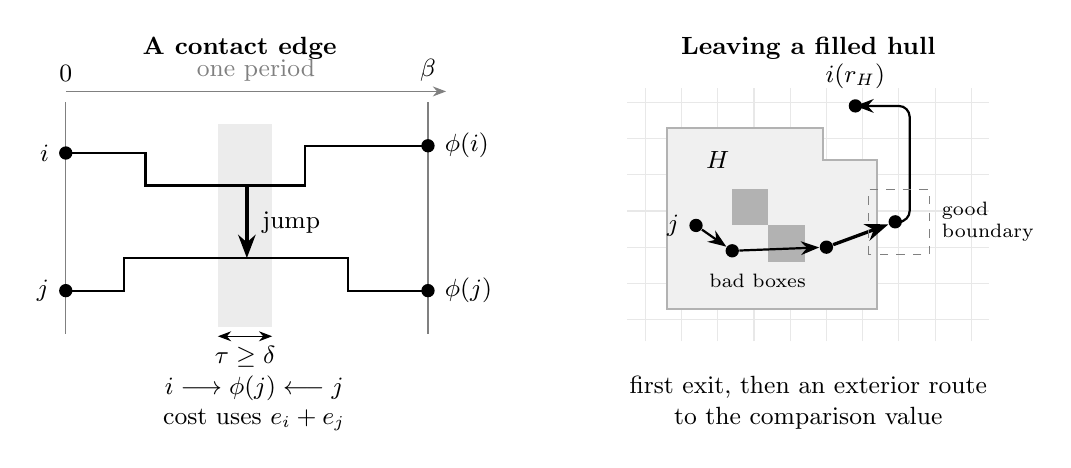
\begin{tikzpicture}[x=.92cm,y=.92cm,>=Stealth,
  every node/.style={font=\small},
  hole/.style={circle,fill=black,inner sep=1.7pt}]
  \begin{scope}
    \node[font=\small\bfseries] at (2.4,4.25) {A contact edge};
    \draw[->,gray] (0,3.65)--(5.25,3.65)
      node[pos=.5,above] {one period};
    \draw[gray] (0,3.5)--(0,.3);
    \draw[gray] (5,3.5)--(5,.3);
    \node[above] at (0,3.65) {$0$};
    \node[above] at (5,3.65) {$\beta$};
    \fill[gray!15] (2.1,.4) rectangle (2.85,3.2);
    \draw[thick] (0,2.8)--(1.1,2.8)--(1.1,2.35)
      --(3.3,2.35)--(3.3,2.9)--(5,2.9);
    \draw[thick] (0,.9)--(.8,.9)--(.8,1.35)
      --(3.9,1.35)--(3.9,.9)--(5,.9);
    \node[hole,label=left:$i$] at (0,2.8) {};
    \node[hole,label=left:$j$] at (0,.9) {};
    \node[hole,label=right:$\phi(i)$] at (5,2.9) {};
    \node[hole,label=right:$\phi(j)$] at (5,.9) {};
    \draw[very thick,->] (2.5,2.35)--(2.5,1.35);
    \node[right] at (2.58,1.84) {jump};
    \draw[<->] (2.1,.27)--(2.85,.27)
       node[midway,below] {$\tau\ge\delta$};
    \node[align=center] at (2.6,-.65)
       {$i\longrightarrow\phi(j)\longleftarrow j$\\
        cost uses $e_i+e_j$};
  \end{scope}
  \begin{scope}[shift={(8.0,0)}]
    \node[font=\small\bfseries] at (2.25,4.25)
       {Leaving a filled hull};
    \draw[step=.5,gray!18] (-.25,.2) grid (4.75,3.7);
    \filldraw[fill=gray!12,draw=gray!60,thick]
       (.3,.65)--(3.2,.65)--(3.2,2.7)--(2.45,2.7)
       --(2.45,3.15)--(.3,3.15)--cycle;
    \node at (1,2.7) {$H$};
    \fill[gray!60] (1.2,1.8) rectangle (1.7,2.3);
    \fill[gray!60] (1.7,1.3) rectangle (2.2,1.8);
    \node[font=\scriptsize,align=center] at (1.55,1.03)
      {bad boxes};
    \node[hole,label=left:$j$] (j) at (.7,1.8) {};
    \node[hole] (v1) at (1.2,1.45) {};
    \node[hole] (v2) at (2.5,1.5) {};
    \node[hole] (v3) at (3.45,1.85) {};
    \draw[thick,->] (j)--(v1);
    \draw[thick,->] (v1)--(v2);
    \draw[very thick,->] (v2)--(v3);
    \draw[rounded corners,thick,->]
      (v3)--(3.65,1.85)--(3.65,3.45)--(2.9,3.45);
    \node[hole,label=above:$i(r_H)$] at (2.9,3.45) {};
    \draw[gray,dashed] (3.08,1.4) rectangle (3.92,2.3);
    \node[font=\scriptsize,align=left,anchor=west]
      at (3.96,1.85) {good\\boundary};
    \node[align=center] at (2.25,-.65)
      {first exit, then an exterior route\\
       to the comparison value};
  \end{scope}
\end{tikzpicture}
\caption{Two parts of the hole comparison, drawn schematically.
Left: a fresh walk jumps between skeleton lines during a contact
interval.  Comparing both cut values through $u_{\phi(j)}$ charges
energy only to the cut starts $i,j$.
Right: a path in $\Gamma$ first exits a filled coarse hull.
Clearance makes its crossing box good; the absence of long mark paths
then confines the whole exiting link near that box.  A surviving
exterior-boundary route leads to $i(r_H)$, which defines $U_B$ on
the hull.  Gray squares indicate bad boxes; the larger gray region
represents the filled hull, with distances and thicknesses not to scale.}
\label{fig:holes-comparison}
\end{figure}

\FloatBarrier

\subsection{Energy, exceptional sets, and the final estimate}

The construction has supplied a bounded comparison function on each
usable cell.  Its lattice gradients are controlled by the total
traversal energy, and a hole fails to match that function only near a
short-time flag or in a small closed class.  We now sum these three
contributions and choose the auxiliary scales.

\begin{lemma}[Cellwise approximation of the resolvent]
\label{lem:cell-resolvent}
There are random numbers $c_B\in[-1,1]$, one per cell, such that
\begin{equation}\label{eq:cell-resolvent}
 \E\sum_B\sum_{\substack{i\in\mathcal H\\x_i\in B}}
        (u_i-c_B)^2\le C_\beta N R^{-1/20}.
\end{equation}
\end{lemma}

\begin{proof}
On a usable cell let $c_B=|B|^{-1}\sum_{x\in B}U_B(x)$; on an
unusable cell put $c_B=0$.  The rectangular lattice Poincar\'e
inequality, whose constant is at most $CR^2$ for the stated side
lengths, gives
\[
 \sum_{x\in B}|U_B(x)-c_B|^2
 \le CR^2\sum_{\substack{\{x,x'\}\subset B\\|x-x'|_1=1}}
                  |U_B(x)-U_B(x')|^2.
\]
It holds in the chosen lift, also for a cell covering an entire
coordinate circle: only the internal rectangle edges are needed.
Use Lemma~\ref{lem:hull-comparison} both here and for the
nonexceptional differences $u_i-U_B(x_i)$.  There are at most
$\ell$ holes above a site.  In summing all the local energy
sums, any fixed torus $e_i$ occurs at most $C_\beta n^3$ times,
since the original fine sites, over all cells, partition the torus.
Periodic copies used to construct the windows do not add summation
sites.  Equation~\eqref{eq:traversal-energy} therefore bounds these
contributions by
\[
 C_\beta R^2n^9\delta^{-1}qN.
\]

All remaining squared differences are at most four.  A fixed fine
site has at most $Cn^3$ boxes in its short-flag neighborhood; its
exceptional probability is at most $C_\beta n^3\delta$ by
Lemma~\ref{lem:bad-box-tail}.  The total number of holes in
$\Gamma$-components of size at most $C_\beta n^3$ is at most
$C_\beta n^3$ times the number of components, whose expectation
is bounded by \eqref{eq:component-count}.  Finally sum
\eqref{eq:unusable-cell} with weights at most $\ell|B|$.
Together these estimates give
\begin{equation}\label{eq:comparison-errors}
 \frac1N\E\sum_B\sum_{\substack{i\in\mathcal H\\x_i\in B}}
      (u_i-c_B)^2
 \le C_\beta\left(
 R^2n^9\delta^{-1}q+n^3\delta+n^3q
                   +R^3e^{-cn^{\lambda_1}}\right).
\end{equation}

Take now
\[
 \delta=R^{-1/8},\qquad n=\lceil R^{1/200}\rceil.
\]
At fixed $\beta$, sufficiently large $R$ meets all preceding
smallness conditions, including $10^6dn\le R\le L$, and the
short-flag threshold in Lemma~\ref{lem:bad-box-tail}.  The first
three terms on the right of \eqref{eq:comparison-errors} are,
respectively,
\[
 O(R^{-33/100}),\qquad O(R^{-11/100}),\qquad
 O(R^{-497/200}).
\]
The fourth is smaller than any negative power of $R$.  This proves
\eqref{eq:cell-resolvent} with the stated, nonoptimal exponent.
\end{proof}

\begin{proof}[Proof of Proposition~\ref{prop:weak-field}]
The partition has at most $CV/R^3$ cells and each has volume
comparable to $R^3$.  Lemmas~\ref{lem:cell-resolvent}
and~\ref{lem:hole-cancellation}, together with $|c_B|\le1$,
give
\begin{align*}
 \E\bigl|\ip{f_{\mathcal H}}{u}\bigr|
 &\le \E\sum_B\sum_{i\in\mathcal H,\,x_i\in B}|u_i-c_B|
       +\sum_B\E\left|\sum_{i\in\mathcal H,\,x_i\in B}f_i\right|\\
 &\le C_\beta N R^{-1/40}
          +CV(qR^3)^{-1/2}.
\end{align*}
In \eqref{eq:transverse-resolvent}, add the diagonal terms inside
the resolvent sum and discard their nonnegative subtraction.
Since $u=qD^{-1}f_{\mathcal H}$, this yields
\[
 \frac qV\langle D_f^2\rangle_b
 \le \frac{qN}{4V}+
       \frac1{2V}\E\bigl|\ip{f_{\mathcal H}}{u}\bigr|
 \le C_\beta\bigl(q+R^{-1/40}+R^{-1/4}\bigr).
\]
This is \eqref{eq:weak-field}.  The assumptions needed for the
sparse-pin estimate hold because $q=R^{-5/2}\ge L^{-5/2}$ and
the lower bound on $R$ can include $L_*(\beta)$.
\end{proof}

\section{Removing the field and comparing spatial scales}
\label{sec:zero-field}

Proposition~\ref{prop:weak-field} controls an ordinary transverse square in
a small positive field.  We first turn this estimate into an exponential
bound at zero field.  The bound is weak for one prescribed test, but it
holds uniformly over enough tests to compare magnetization averages in a
cell with those in its children.  Throughout this section, $\beta$ is
sufficiently large and fixed.

\subsection{Curvature of a logarithmic Laplace transform}

The analytic step uses the following strip lemma.  Its positivity is
essential: small curvature at the origin will then control curvature on
a real interval whose length grows logarithmically with the spatial
scale.

\begin{lemma}[Strip curvature]\label{lem:strip-curvature}
Let $F$ be holomorphic on $\{z\in\C:|\Ima z|<a_0\}$, real and even on
the real axis, with $F(0)=0$.  Suppose that, for some $K<\infty$,
\[
  0\le F(x)\le K|x|,
  \qquad \Rea F(x+iy)\le F(x)
  \quad(x\in\R,\ |y|<a_0).
\]
For each $a\in(0,a_0)$ there is a strictly positive Schwartz function
$J_a$ such that, with $g_a(x)=F(x)-\Rea F(x+ia)$,
\begin{equation}\label{eq:strip-convolution}
 F''=J_a*g_a,
 \qquad
 J_a=\frac{2}{a^2}(h_a*h_a),
 \qquad
 h_a(x)=\frac{\pi}{2a}\sech^2\!\left(\frac{\pi x}{a}\right).
\end{equation}
In particular, with $c_a=2\pi/a$,
\begin{equation}\label{eq:strip-curvature-growth}
  0\le F''(x)\le e^{c_a|x|}F''(0),
  \qquad
  F(x)\le \frac{F''(0)}{c_a^2}
       \bigl(e^{c_a|x|}-1-c_a|x|\bigr).
\end{equation}
\end{lemma}

\begin{proof}
Put $u(x,y)=\Rea F(x+iy)$.  Schwarz reflection makes $u$ even in $y$.
We first justify Fourier transformation in the unbounded horizontal
direction.  Fix $a'<a_0$.  Around each vertical segment
$\{x+iy:|y|\le a'\}$ choose a rectangle of fixed width and height
strictly inside the strip.  On that rectangle the harmonic function
$M_x-u$, with $M_x=C(1+|x|)$ and $C$ sufficiently large, is positive.
Its value at $(x,0)$ is at most $C(1+|x|)$ because $F(x)\ge0$.
Harnack's inequality, followed by interior derivative estimates, gives
\[
 |u(x,y)|+|\partial_x^j\partial_y^k u(x,y)|
      \le C_{a',j,k}(1+|x|),\qquad |y|\le a',
\]
where for derivatives one first uses a slightly larger closed substrip.
Thus $u(\cdot,y)$ and all derivatives needed below are tempered
distributions, smoothly depending on $y$.

Use the Fourier convention $\widehat h(\xi)=\int e^{-ix\xi}h(x)\dd x$.
The harmonic equation becomes
$\partial_y^2\widehat u=\xi^2\widehat u$.  This equation is solved
\emph{locally in frequency}: multiply by a smooth function of compact
support in $\xi$ and solve the resulting distribution-valued ordinary
differential equation.  Multiplication by its fundamental matrix is
then legitimate, since $\xi$ remains in a compact set.  The initial
data are $\widehat u(\xi,0)=\widehat F(\xi)$ and
$\partial_y\widehat u(\xi,0)=0$.  Consequently
\[
 \widehat u(\xi,a)=\cosh(a\xi)\widehat F(\xi)
\]
on every compact frequency interval.  We do not multiply an arbitrary
tempered distribution globally by the exponentially growing function
$\cosh(a\xi)$.

The smooth function
\[
 m_a(\xi)=\frac{\xi^2}{\cosh(a\xi)-1},
 \qquad m_a(0)=\frac{2}{a^2},
\]
is Schwartz.  The preceding local identity gives
$m_a\widehat g_a=-\xi^2\widehat F$ on every compact frequency interval,
and hence as tempered distributions.  To identify its inverse Fourier
transform, the substitution $r=e^{2\pi x/a}$ and the beta integral give
\[
 \widehat h_a(\xi)
 =\int_0^\infty\frac{r^{-ia\xi/(2\pi)}}{(1+r)^2}\dd r
 =\frac{a\xi/2}{\sinh(a\xi/2)}.
\]
The value at zero is understood by continuity.  It follows that
$m_a=(2/a^2)\widehat h_a^{\,2}$, proving
\eqref{eq:strip-convolution}.  The convolution is an ordinary convergent
integral because $g_a$ has polynomial growth.  Its distributional
identity therefore holds pointwise.

Both $h_a$ and $J_a$ are strictly positive Schwartz functions.  Moreover,
$|h_a'|\le c_a h_a$, so differentiation under the convolution gives
$|J_a'|\le c_a J_a$.  Hence
$J_a(x-t)\le e^{c_a|x|}J_a(-t)$.  Since $g_a\ge0$, integration proves
the first inequality in \eqref{eq:strip-curvature-growth}.  Integrating
twice, using $F(0)=F'(0)=0$ and evenness, proves the second.
\end{proof}

\subsection{A zero-field exponential bound}

\begin{proposition}\label{prop:zero-field}
Fix $S$ and a sufficiently large finite $\beta$.  There are
$R_0=R_0(S,\beta)$, $C_\beta<\infty$, and $\kappa>0$ with the following
property.  Let $L\ge R\ge R_0$, with $L$ even, and partition $\Lambda_L$
into rectangular cells whose side lengths lie in $[R/2,4R]$.  If
$f:\Lambda_L\to[-1,1]$ has sum zero on every cell, then, for
$q=R^{-5/2}$, $b=-\log(1-q)$, and any spin component $a$,
\begin{equation}\label{eq:zero-exp}
 \log\left\langle
   \exp\left(bx\sum_{z\in\Lambda_L}f_zS_z^a\right)
 \right\rangle
 \le C_\beta bV,
 \qquad x\in\R,\quad |x|\le\kappa\log R.
\end{equation}
Consequently there are $A_\beta,c>0$ such that the spectral measurement
of $D_f=\sum_z f_zS_z^a$ in the zero-field state satisfies
\begin{equation}\label{eq:zero-tail}
 \PP\left\{|D_f|>\frac{A_\beta V}{\log R}\right\}
       \le 2e^{-cbV}.
\end{equation}
All bounds are uniform over the indicated partitions and tests.
\end{proposition}

\begin{proof}
It suffices first to take $a=3$ and put the field in direction $Y$.
Write $D_f=\sum_z f_zZ_z$ and define
\[
 F(z)=\frac{1}{bV}\log\langle e^{bzD_f}\rangle_b.
\]
Since $[H_0,M_L^2]=0$, cyclicity of the trace gives
\[
 \langle e^{bzD_f}\rangle_b
 =\frac{\Tr_{\rm phys}
       \bigl(e^{H_0}e^{bM_L^2/2}e^{bzD_f}e^{bM_L^2/2}\bigr)}
       {\Tr_{\rm phys}e^{H_0+bM_L^2}}.
\]
The middle three factors form the restriction of a tensor product of
single-slot sandwich matrices.  Lemma~\ref{lem:strip-maps}, applied to
$e^{bs^2/2}e^{bzf_zs^3}e^{bs^2/2}$, and
Lemma~\ref{lem:trace-zero-free} show that the expression inside the
logarithm has no zeros in a fixed strip $|\Ima z|<a_0$.
Here $R_0$ is large enough that $b\le b_*$ from
Lemma~\ref{lem:strip-maps}.  Choose the analytic logarithm that is real
on the real axis and vanishes at zero.

This is the logarithm of an \emph{ordinary} Laplace transform: the
spectral measure of $D_f$ in the tilted Gibbs state is a probability
measure, even though $D_f$ need not commute with its density matrix.
Rotation by $\pi$ around the field axis makes this measure even.
Therefore $F$ is even, $F(x)\ge0$, and, since $\|D_f\|\le SV$,
\[
 \Rea F(x+iy)\le F(x)\le S|x|.
\]
In particular,
\[
 F''(0)=\frac bV\Var_b(D_f)
       =\frac bV\langle D_f^2\rangle_b
       \le C_\beta R^{-\eta}
\]
by Proposition~\ref{prop:weak-field}, with $\eta=1/40$, and
$b/q\le2$ for large $R$.
This derivative is an ordinary variance, not the Duhamel covariance
obtained by perturbing the Hamiltonian inside its exponential.

Fix $a\in(0,a_0)$ in Lemma~\ref{lem:strip-curvature}.  Choose
$\kappa>0$ so that $c_a\kappa<\eta/2$.  Equation
\eqref{eq:strip-curvature-growth} then gives, uniformly over our tests,
\[
 0\le F(x)\le C_\beta R^{-\eta/2},
 \qquad |x|\le\kappa\log R.
\]
To remove the field, let $\gamma_0$ and $\gamma_b$ be the normalized
zero-field and tilted density matrices.  Since $H_0$ commutes with
$M_L^2$ and $\|M_L^2\|\le SV$,
\[
 \gamma_0\le e^{2bSV}\gamma_b.
\]
Taking the trace against the positive operator $e^{bxD_f}$ costs at
most $2bSV$ in its logarithm and proves \eqref{eq:zero-exp} for $a=3$.
Rotation invariance of $\gamma_0$ gives every common axis.
Finally, exponential Markov at $x=\pm\kappa\log R$, with
$\kappa A_\beta>C_\beta+c$, proves \eqref{eq:zero-tail}.
\end{proof}

\subsection{Comparison through nested partitions}

For a rectangular cell $C$ and an axis $a$, write
\[
 \overline S_C^a=\frac1{|C|}\sum_{x\in C}S_x^a.
\]
All averages in a single fixed axis commute.  The next proposition
compares their ordinary squares; it makes no joint-measurement assertion
about the three spin components.

\begin{proposition}\label{prop:scale-comparison}
Fix $S$ and a sufficiently large finite $\beta$.  For every sufficiently
large fixed $R_*$ and all sufficiently large even $L$, there is a
deterministic rectangular partition $\mathcal P_*(L)$ of $\Lambda_L$
whose side lengths lie in $[R_*/2,4R_*^{10/9}]$ and such that, for
$a=1,2,3$,
\begin{equation}\label{eq:spatial-comparison}
 \frac1V\sum_{C\in\mathcal P_*(L)}|C|
       \left\langle(\overline S_C^a)^2\right\rangle
 \le
       \left\langle(M_L^a/V)^2\right\rangle
       +\frac{C_\beta}{\log R_*}+o_L(1).
\end{equation}
Here $o_L(1)\to0$ at fixed $R_*$ and $\beta$.
\end{proposition}

\begin{proof}
Set $R_0=L$ and $R_{j+1}=R_j^{9/10}$, and stop at the largest $n$
for which $R_n\ge R_*$.  Starting with the one-cell partition, construct
nested rectangular partitions $\mathcal P_j$ with cell sides in
$[R_j/2,4R_j]$.  For example, subdivide each coordinate interval of a
parent into nearly equal integer intervals of length comparable to
$R_{j+1}$.  The ratios $R_j/R_{j+1}$ are large once $R_*$ is large,
so every such subdivision meets the stated bounds.  The final scale
satisfies $R_*\le R_n<R_*^{10/9}$.

Fix an axis and perform its simultaneous site-spin measurement.
Let $D(C)$ denote the measured value of $\overline S_C^a$.  For one
refinement, put $R=R_j$, $r=R_{j+1}$, and define
\[
 T_j=\frac1V\sum_{B\in\mathcal P_j}
             \sum_{\substack{C\in\mathcal P_{j+1}\\C\subset B}}
               |C|\,|D(C)-D(B)|.
\]
To express $T_j$ through the tests of Proposition~\ref{prop:zero-field},
assign a sign $\sigma_C\in\{-1,1\}$ to every child and put
\[
 \bar\sigma_B=\frac1{|B|}\sum_{C\subset B}|C|\sigma_C,
 \qquad
 f_x=\frac{\sigma_C-\bar\sigma_B}{2}
       \quad(x\in C\subset B).
\]
Then $|f_x|\le1$ and $\sum_{x\in B}f_x=0$.  Direct expansion gives
\[
 \sum_x f_xS_x^a
   =\frac12\sum_{B,C\subset B}|C|\sigma_C\bigl(D(C)-D(B)\bigr)
\]
in this measurement.  Maximizing over the signs therefore gives $VT_j/2$.
There are at most $\exp(CV/r^3)$ sign choices, because every child has
volume at least $(r/2)^3$.  Applying \eqref{eq:zero-tail} to each test
and taking a union bound yields
\[
 \PP\{T_j>2A_\beta/\log R\}
 \le 2\exp\{CV R^{-27/10}-cbV\}
 \le 2\exp(-c'VR^{-5/2}).
\]
The last inequality holds uniformly after increasing $R_*$, since
$b\ge R^{-5/2}$ and $R^{-27/10}=o(R^{-5/2})$.

As $|D(C)-D(B)|\le2S$, this also bounds the expected weighted square
increment:
\[
 \E\left[\frac1V\sum_{B,C\subset B}|C|
                 (D(C)-D(B))^2\right]
 \le \frac{C_\beta}{\log R_j}
       +C\exp(-c'VR_j^{-5/2}).
\]
The squares telescope exactly, because $D(B)$ is the weighted mean of
its children's averages:
\[
 \sum_{C\in\mathcal P_{j+1}}|C|D(C)^2
 -\sum_{B\in\mathcal P_j}|B|D(B)^2
 =\sum_{B,C\subset B}|C|(D(C)-D(B))^2.
\]
Now
$\sum_{j<n}(\log R_j)^{-1}\le C/\log R_*$, whereas
$VR_j^{-5/2}\ge L^{1/2}$ and $n=O(\log\log L)$.
Summing the expected increments proves \eqref{eq:spatial-comparison}
with $\mathcal P_*(L)=\mathcal P_n$.  The deterministic construction
works for all three axes.
\end{proof}

\section{Equilibrium states and vanishing replica cross terms}
\label{sec:equilibrium}

The spatial estimate has a second use besides comparing block averages:
it removes certain couplings between independent replicas at a pressure
tangent.  We give the variational framework first, including the precise
order of limits needed for this deduction.  The underlying lattice is
now $\Z^3$, with the spin-$S$ matrix algebra at each site.  A state is a
consistent family of density matrices on finite sets, or equivalently
a positive normalized functional on the norm closure of the local
matrix algebras.  Local convergence means convergence on every local
observable.  Write $\mathcal S_{\rm TI}$ for the compact convex set of
translation-invariant states, and $\tau_x$ for translation by $x$.

\subsection{The variational principle and its tangents}

For a density matrix $\rho$, let
$\mathsf S(\rho)=-\Tr(\rho\log\rho)$.  If $Q_n=\{0,\ldots,n-1\}^3$
and $\omega\in\mathcal S_{\rm TI}$, its mean entropy and unperturbed
interaction expectation per site are
\[
 \mathfrak s(\omega)=\lim_{n\to\infty}\frac{\mathsf S(\omega_{Q_n})}{|Q_n|},
 \qquad
 e_0(\omega)=\beta\sum_{r=1}^3
                     \omega(\mathbf S_0\cdot\mathbf S_{e_r}).
\]
For a self-adjoint local observable $a$, let
$A_L=\sum_{x\in\Lambda_L}\tau_x(a)$, interpreted periodically for $L$
larger than its support, and set
\[
 P_a(t)=\lim_{L\to\infty}\frac1V
                   \log\Tr e^{H_0+tA_L},\qquad t\in\R.
\]
The limit uses even $L$, as elsewhere.  Finite range and boundedness
make free and periodic boundary conditions equivalent for this limit:
the difference of their exponents has norm $O(L^2)$.

The following standard variational facts are recalled with proofs to
specify the state space on which the later tangent is taken; see
\cite[Theorems~2--3]{LanfordRobinson1968Entropy} and
\cite[Theorem~3]{LanfordRobinson1968Spin}.

\begin{proposition}\label{prop:variational-framework}
The mean entropy exists on $\mathcal S_{\rm TI}$, is upper
semicontinuous and affine, and
\begin{equation}\label{eq:variational-pressure}
 P_a(t)=\max_{\omega\in\mathcal S_{\rm TI}}
       \{\mathfrak s(\omega)+e_0(\omega)+t\omega(a)\}.
\end{equation}
In particular, writing $P_0=\beta p_{S,\beta}(0)$, the set
\[
 \mathcal E_\beta=
 \{\omega\in\mathcal S_{\rm TI}:
            \mathfrak s(\omega)+e_0(\omega)=P_0\}
\]
is a nonempty compact face of $\mathcal S_{\rm TI}$.  Every local limit
of periodic zero-field Gibbs states belongs to $\mathcal E_\beta$,
and
\begin{equation}\label{eq:pressure-tangent}
 P_a'(0+)=\max_{\omega\in\mathcal E_\beta}\omega(a).
\end{equation}
The extreme points of $\mathcal E_\beta$ are precisely its states that
are extreme in $\mathcal S_{\rm TI}$; we call these states ergodic.
\end{proposition}

\begin{proof}
Tile a large cube by translates of $Q_n$ and a remainder of vanishing
relative volume.  Entropy subadditivity and the bound
$\mathsf S(\rho_B)\le |B|\log(2S+1)$ show that
\[
 \mathfrak s(\omega)
       =\inf_{n\ge1}\frac{\mathsf S(\omega_{Q_n})}{|Q_n|}.
\]
This proves existence and upper semicontinuity, since each finite-volume
entropy is continuous.  For a mixture $\rho=\lambda\rho_1+(1-\lambda)\rho_2$,
the entropy lies between
$\lambda\mathsf S(\rho_1)+(1-\lambda)\mathsf S(\rho_2)$ and this quantity
plus the binary entropy of $\lambda$.  Division by volume proves
affinity of $\mathfrak s$.

Apply the finite-dimensional Gibbs variational principle to the
restriction of any $\omega\in\mathcal S_{\rm TI}$ to a large cube.
Boundary terms are $o(V)$ in norm, so
$P_a(t)\ge\mathfrak s(\omega)+e_0(\omega)+t\omega(a)$.
Conversely, choose a locally convergent subsequence of periodic Gibbs
states for $H_0+tA_L$, with limit $\omega$.  The limit is translation
invariant, and local interaction expectations converge.  Tiling the
large cubes by fixed cubes $Q_n$ gives
\[
 \limsup_{L\to\infty}\frac{\mathsf S(\gamma_{L,t})}{V}
 \le \frac{\mathsf S(\omega_{Q_n})}{|Q_n|}
 \quad\hbox{for every }n.
\]
Letting $n\to\infty$ and using the exact finite-volume Gibbs identity
gives the reverse variational inequality.  At $t=0$ this argument also
proves the assertion about every periodic Gibbs local limit.  Compactness,
upper semicontinuity, and affinity show that $\mathcal E_\beta$ is a
nonempty compact face; the assertion about its extreme points follows
from the definition of a face.

For completeness, a maximizer $\omega_t$ in
\eqref{eq:variational-pressure}, with $t>0$, satisfies
\[
 \max_{\omega\in\mathcal E_\beta}\omega(a)
 \le\frac{P_a(t)-P_0}{t}\le\omega_t(a).
\]
As $t\downarrow0$, upper semicontinuity shows that every local limit
of $\omega_t$ belongs to $\mathcal E_\beta$: its unperturbed variational
value tends to $P_0$, since $|\omega_t(a)|\le\|a\|$.
Taking a convergent subsequence proves \eqref{eq:pressure-tangent}.
\end{proof}

In the field direction $Y$, the exponent-normalized pressure is
$\beta p_{S,\beta}(b/\beta)$.  Thus
\begin{equation}\label{eq:magnetization-max}
 m=\max_{\omega\in\mathcal E_\beta}\omega(Y_0).
\end{equation}
Rotation invariance gives the same maximum in every unit direction.
Consequently the vector
$\mathbf m(\omega)=(\omega(X_0),\omega(Y_0),\omega(Z_0))$ has length
at most $m$ for every $\omega\in\mathcal E_\beta$.  The face maximizing
$\omega(Y_0)$ has an extreme point, so an ergodic equilibrium state
attains $m$.  Section~\ref{sec:pressure} will prove that every ergodic
equilibrium state has this same magnetization magnitude.

The following mean-ergodic consequence of extremality is standard for
asymptotically commuting lattice translations; see
\cite[Theorem~3]{KastlerRobinson1966}.

\begin{lemma}[Ergodic averages]\label{lem:ergodic-variance}
If $\omega$ is an extreme translation-invariant state and $A$ is a
self-adjoint local observable, then
\[
 \lim_{n\to\infty}
 \omega\left[\left(
      \frac1{|Q_n|}\sum_{x\in Q_n}\tau_x(A)-\omega(A)\1
                   \right)^2\right]=0.
\]
\end{lemma}

\begin{proof}
After shifting and scaling, assume $0\le A\le\1$, and denote its
average by $\bar A_n$.  In the Hilbert space of the state, translations
are commuting unitaries.  The mean ergodic theorem makes
$\bar A_n\Omega$ converge to a vector $\eta$, where $\Omega$ represents
the state.  Hence $\lambda(C)=\lim_n\omega(C\bar A_n)$ exists for every
local $C$.

For local $C\ge0$, locality gives
$\|[C^{1/2},\bar A_n]\|\to0$.  Therefore
$\lambda(C)=\lim_n\omega(C^{1/2}\bar A_nC^{1/2})$, and
$0\le\lambda(C)\le\omega(C)$.  The functional extends continuously,
is translation invariant by the boundary-to-volume estimate for the
averages, and satisfies $\lambda(\1)=\omega(A)$.  Extremality of
$\omega$ now gives $\lambda=\omega(A)\omega$: otherwise its normalized
parts in $\omega=\lambda+(\omega-\lambda)$ would give a nontrivial
convex decomposition into translation-invariant states.  Testing on
the dense set of local vectors identifies $\eta=\omega(A)\Omega$,
which is the asserted variance convergence.
\end{proof}

\subsection{Products of zero-sum observables in distinct replicas}

Take $j$ copies of the spin system, with superscripts $[r]$ denoting
the replica.  The unperturbed exponent is
$\sum_{r=1}^jH_0^{[r]}$, and its pressure is $jP_0$.  Every
translation-invariant equilibrium state for this interaction has each
marginal in $\mathcal E_\beta$.  Indeed, entropy subadditivity between
replicas bounds its variational value by the sum of the marginal
variational values, each at most $P_0$; equality of the total forces
equality for each marginal.  Conversely, products of states in
$\mathcal E_\beta$ are replicated equilibrium states, because their
entropies and interaction expectations add.

For real coefficients $v_i$ on finitely many qubit slots, define
\[
 D_v^a=\sum_i v_i s_i^a,
 \qquad B_v^a=P_*D_v^aP_*
\]
as a physical local operator.  On a site's symmetric subspace,
$P_*s_{(x,k)}^aP_*=S_x^a/\ell$.  Thus
\begin{equation}\label{eq:compressed-zero-sum}
 B_v^a=\sum_x c_x S_x^a,
 \qquad c_x=\frac1\ell\sum_{k=1}^{\ell}v_{(x,k)},
 \qquad \sum_xc_x=0\quad\hbox{if }\sum_iv_i=0.
\end{equation}
The next lemma concerns products of these \emph{compressed} operators
in different replicas.  It does not identify $P_*(D_v^a)^2P_*$ with
$(B_v^a)^2$.

\begin{lemma}[Replica cross terms]\label{lem:replica-cross}
Fix $S$ and a sufficiently large finite $\beta$.  Let $\omega$ be any
translation-invariant equilibrium state of $j$ unperturbed replicas.
For distinct replicas $r,s$, axes $a,b$, and finitely supported real
slot coefficients $v,w$ with $\sum_i v_i=\sum_i w_i=0$,
\[
 \omega\bigl((B_v^a)^{[r]}(B_w^b)^{[s]}\bigr)=0.
\]
The same holds for every finite linear combination of translates of
such products.
\end{lemma}

\begin{proof}
Write $O=(B_v^a)^{[r]}(B_w^b)^{[s]}$ and choose a fixed cube of side
$d$ containing both spatial supports.  Let $\rho_L$ be the restriction
of $\omega$ to a cube of side $L$, and let $\gamma_L$ be the product
of the $j$ periodic zero-field Gibbs density matrices on that cube.
With $D(\rho\Vert\gamma)=\Tr\rho(\log\rho-\log\gamma)$,
\begin{equation}\label{eq:replica-relative-entropy}
 \frac1V D(\rho_L\Vert\gamma_L)\longrightarrow0.
\end{equation}
Indeed, expanding $\log\gamma_L$ gives $j$ times the finite-volume
pressure minus the entropy density and interaction density of
$\rho_L$.  Their limits cancel by the equilibrium variational identity;
periodic bonds at the boundary change the interaction by $o(V)$.

Fix an integer $R\ge d$ and take $L$ through even multiples of $R$.
Partition the cube into cells of side $R$, and let $\mathcal T$ be the
translations of the chosen support cube lying wholly within individual
cells.  In particular,
\[
 \frac{|\mathcal T|}{V}
       =\left(\frac{R-d+1}{R}\right)^3.
\]
Write $B_v^a=\sum_xc_xS_x^a$ and $B_w^b=\sum_xd_xS_x^b$, as in
\eqref{eq:compressed-zero-sum}.  Choose
$C_O\ge\max\{1,S\|c\|_1\|d\|_1\}$ and put
\[
 O'=\frac1{C_O}\sum_{y\in\mathcal T}\tau_y(O).
\]
All operators in this sum can be measured simultaneously, using axis
$a$ in replica $r$ and axis $b$ in replica $s$.  Conditional on any
outcome in replica $s$, denote the value of
$\tau_y(B_w^b)^{[s]}$ by $b_y$, so $|b_y|\le S\|d\|_1$.
As a function of the first replica's outcomes, $O'$ is then
$\sum_z f_zS_z^a$, where
\[
 f_z=\frac1{C_O}\sum_{y\in\mathcal T}c_{z-y}b_y.
\]
These coefficients have absolute value at most one.  Their sum in each
cell vanishes, since each translated support stays in that cell and
$\sum_xc_x=0$.  Independence of the replicas under $\gamma_L$ and
Proposition~\ref{prop:zero-field}, applied conditionally, therefore give
\begin{equation}\label{eq:replica-exponential}
 \log\Tr(\gamma_Le^{\pm\theta O'})\le C_\beta bV,
 \qquad
 b=-\log(1-R^{-5/2}),\quad\theta=\kappa b\log R.
\end{equation}

For any self-adjoint $K$, the Gibbs variational principle followed by
the Golden--Thompson inequality \cite{Golden1965,Thompson1965} gives
\[
 \Tr(\rho_LK)
 \le D(\rho_L\Vert\gamma_L)
       +\log\Tr e^{\log\gamma_L+K}
 \le D(\rho_L\Vert\gamma_L)+\log\Tr(\gamma_Le^K).
\]
Use $K=\theta O'$ or $K=-\theta O'$ according to the sign of
$\omega(O)$.  Translation invariance and
\eqref{eq:replica-exponential} yield
\[
 \theta\frac{|\mathcal T|}{C_O}|\omega(O)|
 \le D(\rho_L\Vert\gamma_L)+C_\beta bV.
\]
First let $L\to\infty$ at this fixed $R$; this order is required because
the entropy density in \eqref{eq:replica-relative-entropy} has no rate.
For large $R$, $|\mathcal T|/V$ is bounded below, and we obtain
$|\omega(O)|\le C_{\beta,O}/\log R$.  Letting $R\to\infty$ proves the
claim.  Linearity gives the final assertion.
\end{proof}

Thus, for a finite-range replica perturbation that is a sum of
single-replica terms and the cross terms in
Lemma~\ref{lem:replica-cross}, its pressure tangent depends only on
the single-replica terms.  The construction in the next section uses
this fact to study negative squares of block magnetizations.

\section{Pressure tangents and the equilibrium magnetization radius}
\label{sec:pressure}

The variational principle bounds the magnetization of every state in
$\mathcal E_\beta$ by $m$.  We now prove that every ergodic member has
magnetization of length exactly $m$.  The obstruction to a smaller radius
will be analyticity of certain pressure tangents.  To obtain that
analyticity, we construct random transfer matrices whose traces are
nonzero before taking expectations; Lemma~\ref{lem:replica-cross} then
identifies the pressure tangents of their moments.

For an integer $r\ge2$, write $C_r=\{0,\ldots,r-1\}^3$, and let
$\mathcal C_r$ denote all its translates, on the lattice or on a sufficiently
large torus.  For any such cube $C$, put
$X_C=\sum_{x\in C}X_x$, and define $Y_C,Z_C$ in the same way.  Fix
$B\ge2$ and $W\ge2B$.  We will choose a constant $D_B>0$, independent of
$W$, and consider the nonpositive local observable
\begin{equation}
 a_{B,W}=-\frac{Y_{C_B}^2}{B^6}
         -D_B\frac{X_{C_W}^2+Z_{C_W}^2}{W^6}.
 \label{eq:negative-square-local}
\end{equation}
In an ergodic state with magnetization vector $(0,r,0)$, the transverse
term tends to zero as $W\to\infty$ at fixed $B$, while the $Y$ term
tends to $-r^2$ as $B\to\infty$, by
Lemma~\ref{lem:ergodic-variance}.
The periodic sum of $a_{B,W}$ is denoted by
$A_{B,W,L}=\sum_{x\in\Lambda_L}\tau_x(a_{B,W})$.  Define
\begin{equation}
 s_{B,W}(x)=\max_{\omega\in\mathcal E_\beta}
       \{\omega(a_{B,W})+x\omega(Y_0)\},\qquad x\in\R.
 \label{eq:square-tangent}
\end{equation}
This function is convex and $S$-Lipschitz.  It is even: a rotation by
$\pi$ around the $X$-axis preserves $a_{B,W}$ and sends $Y_0$ to $-Y_0$.

\begin{proposition}[Harmonic pressure tangent]
\label{prop:harmonic-tangent}
For every integer $B\ge2$ there is $D_B>0$ such that, for every integer
$W\ge2B$, the function in \eqref{eq:square-tangent} has a harmonic
extension $v_{B,W}$ from the positive real axis to
$\mathbb H=\{z\in\C:\Re z>0\}$ satisfying
\begin{equation}
 v_{B,W}(x)=s_{B,W}(x)\quad(x>0),\qquad
 v_{B,W}(z)\le s_{B,W}(\Re z)\quad(z\in\mathbb H).
 \label{eq:harmonic-tangent}
\end{equation}
\end{proposition}

We prove the proposition in the next three subsections.  We first
express the negative squares in
\eqref{eq:negative-square-local} as infinitesimal contributions of real
single-slot matrices, together with a small reduction of the
ferromagnetic coupling.  Shared Gaussian coefficients then turn moments
of the random traces into replicated pressures.  Finally a second-moment
argument selects nonvanishing traces whose logarithms converge to the
required harmonic function.

\subsection{A Laplacian construction for the negative squares}

Recall that there are $\ell=2S$ slots per site and that $P_*$ projects
onto the physical spin space.  For a real vector $v=(v_i)$ on finitely
many slots, write
\[
 D_v^a=\sum_i v_i s_i^a.
\]
Our generators will be $iD_v^2$ and $D_v^1,D_v^3$, with $\sum_i v_i=0$.
All three are real matrices in the $s^3$ basis, and their exponentials
with real coefficients are products of single-slot matrices in
$SL_2(\R)$.  Squaring $iD_v^2$ contributes a negative square in the
$Y$-direction.  The other two generators contribute positive squares;
the reduction of the static coupling will cancel their unwanted
nearest-neighbor coefficients.

All quadratic coefficients below use \emph{ordered} slot pairs:
\[
 (D_v^a)^2=\sum_{i,j}v_iv_j s_i^a s_j^a.
\]
For a cube $C$, let $L_C^{\rm full}$ be the graph Laplacian of the
complete graph on its $\ell|C|$ slots.  Let $L_C^{\rm bond}$ be the
Laplacian with an edge between every pair of slots whose sites are
nearest neighbors inside $C$.  Thus an off-diagonal Laplacian entry is
$-1$ on an edge.  These matrices are extended by zero when used on a
larger slot set.

The bond graph of $C_B$ is connected.  Consequently one can choose
$c_B>0$ so that, for every $C\in\mathcal C_B$,
\begin{equation}
 Q_C=c_B L_C^{\rm bond}-B^{-6}L_C^{\rm full}\ge0.
 \label{eq:small-cube-covariance}
\end{equation}
Indeed, both matrices annihilate the constant vector, and on its
orthogonal complement the bond Laplacian is positive definite while
$L_C^{\rm full}=\ell B^3I$.  Decompose $Q_C$ spectrally as
$\sum_v vv^{\mathsf T}$.  Every vector in this sum is real and has zero
sum; use the generators $iD_v^2$ for this list.

To cancel the remaining static reduction in the $X,Z$ directions, put
$n_{B,W}=(W-B+1)^3$ and, for $C\in\mathcal C_W$, consider
\begin{equation}
 R_C=D_BW^{-6}L_C^{\rm full}
       -\frac{c_B}{n_{B,W}}
          \sum_{\substack{C'\in\mathcal C_B\\C'\subseteq C}}
                      L_{C'}^{\rm bond}.
 \label{eq:large-cube-covariance}
\end{equation}
The constant $D_B$ can be chosen so that $R_C\ge0$ for every $W\ge2B$.
Here is a uniform bound.  Each slot belongs to at most $B^3$ small cubes,
and its degree in each bond graph is at most $6\ell$.  The sum of the
bond Laplacians therefore has norm at most $12\ell B^3$.  Since
$n_{B,W}\ge W^3/8$, the second term in
\eqref{eq:large-cube-covariance} has norm at most
$96c_B\ell B^3/W^3$.  On the zero-sum subspace, the first term is
$D_B\ell/W^3$ times the identity.  Thus, for example,
\begin{equation}
 D_B=96c_BB^3+1
 \label{eq:DB-choice}
\end{equation}
suffices.  Decompose each $R_C$ as $\sum_v vv^{\mathsf T}$ with real
zero-sum vectors, and use both generators $D_v^1$ and $D_v^3$.  Choose
the lists on one cube of each size and translate them.  The resulting
families are translation invariant.

Let $T_{B,L}$ be the physical compression of the static reduction
\begin{equation}
 -c_B\sum_{C\in\mathcal C_B}
     \sum_{\substack{i,j\text{ slots in }C\\
                     x_i,x_j\text{ nearest neighbors}}}
                   \sum_{a=1}^3s_i^a s_j^a,
 \label{eq:static-reduction}
\end{equation}
where the inner sum is ordered.  Each unordered site bond belongs to
$(B-1)B^2$ translates of $C_B$, so
\[
 H_{0,t}:=H_0+tT_{B,L}
   =\bigl(\beta-2tc_B(B-1)B^2\bigr)
                    \sum_{\{x,y\}\text{ bond}}\mathbf S_x\cdot\mathbf S_y.
\]
For fixed $B$ this remains ferromagnetic for all sufficiently small
$t>0$, uniformly in $L>2W$.

Denote all the generators just constructed by $G_\alpha$.  Their
quadratic contribution is compressed \emph{after squaring}:
\begin{equation}
 T_{B,L}+\sum_\alpha P_*G_\alpha^2P_*
       =A_{B,W,L}+C_{B,W}VI
 \label{eq:pulse-identity}
\end{equation}
on physical space, for a real scalar $C_{B,W}$ independent of $L>2W$.
To check the identity, first consider distinct slots $i,j$ in the cube
$C$ under consideration.  If $E_C(i,j)$
is the indicator of an edge of the bond graph, the coefficients from
a small cube in the $Y$-direction are
\[
 \underbrace{-c_BE_C(i,j)}_{\text{static reduction}}
 +\underbrace{\bigl(c_BE_C(i,j)-B^{-6}\bigr)}_{-(Q_C)_{ij}}
 =-B^{-6}.
\]
For either the $X$- or the $Z$-direction, the contribution from a large
cube is
\[
 (R_C)_{ij}=-D_BW^{-6}
       +\frac{c_B}{n_{B,W}}
          \sum_{\substack{C'\in\mathcal C_B\\C'\subseteq C}}E_{C'}(i,j).
\]
Every small cube lies in exactly $n_{B,W}$ large cubes.  After summing
over translates, the second term cancels the static reduction, leaving
the coefficient $-D_BW^{-6}$ on each ordered pair in each large cube.
These are precisely the off-diagonal coefficients of $A_{B,W,L}$.
The remaining terms have $i=j$ and are scalar because
$(s_i^a)^2=I/4$; translation invariance gives the scalar in
\eqref{eq:pulse-identity}.  In particular, the identity does not replace
$P_*G_\alpha^2P_*$ by $(P_*G_\alpha P_*)^2$, which would in general
give different single-replica terms.

\subsection{Nonvanishing random traces and replicated moments}

Fix $B,W$ and a sufficiently small $t>0$.  For an even $L>2W$ and an
integer $k\ge1$, take independent real centered Gaussian variables
$\lambda_{r,\alpha}$, $1\le r\le k$, of variance $2t/k$.  Fix an order
of the generators and define a slot-space layer
\[
 U_r(z)=\left(\prod_\alpha e^{\lambda_{r,\alpha}G_\alpha}\right)
                       e^{(tz/k)\sum_i s_i^2}.
\]
Only the complete layer is compressed.  With all products taken in
their fixed order, define the normalized random entire function
\begin{equation}
 \mathcal Z_{L,k,t}(z)=
 \frac{e^{-tC_{B,W}V}}{\Tr e^{H_0}}
 \Tr_{\rm phys}\prod_{r=1}^k
       \left[e^{H_{0,t}/k}\bigl(P_*U_r(z)P_*\bigr)\right].
 \label{eq:random-partition}
\end{equation}
Gaussian exponential moments ensure that all finite products of these
functions are integrable, locally uniformly in their arguments.

Every realization of \eqref{eq:random-partition} is nonzero on
$\mathbb H$.  Although the pulse supports overlap, their fixed ordered
product is still a tensor product of single-slot matrices: factors on
different slots commute and can be regrouped without changing the
order on any one slot.  All pulse matrices on a slot lie in
$SL_2(\R)$ and hence act as disk automorphisms in the $s^2$ basis, by
Lemma~\ref{lem:strip-maps}.  On every slot the remaining factor $e^{tzs^2/k}$ sends the
closed disk strictly inside the disk when $\Re z>0$.  Their composition
therefore has the strict mapping property of
Lemma~\ref{lem:trace-zero-free}.  To identify the permutation layers,
write $E$ for the full-slot exponential of the static interaction
with time step $1/k$.  It commutes with $P_*$, and cyclicity gives
\[
 \Tr_{\rm phys}\prod_{r=1}^k
       [e^{H_{0,t}/k}(P_*U_r(z)P_*)]
      =\Tr_{\rm slots}\prod_{r=1}^k[(EP_*)U_r(z)].
\]
Each $EP_*$ has nonnegative exchange rates and a symmetric seam, so
it is a permutation layer of the class allowed in that lemma.  The
identity uses $P_*^2=P_*$ and does not require $U_r$ to preserve
physical space.  This proves
samplewise nonvanishing, and in particular
\begin{equation}
 z\longmapsto\frac{1}{tV}\log|\mathcal Z_{L,k,t}(z)|
 \quad\text{is harmonic on }\mathbb H.
 \label{eq:sample-harmonic}
\end{equation}

Complex conjugation has a specific sign here.  The static matrices,
the projections and all pulses are real in the $s^3$ basis, whereas
$s^2$ is purely imaginary.  Therefore, for the \emph{same} Gaussian
sample,
\begin{equation}
 \overline{\mathcal Z_{L,k,t}(z)}
       =\mathcal Z_{L,k,t}(-\overline z).
 \label{eq:sample-conjugation}
\end{equation}
The argument on the right may lie outside $\mathbb H$; the function is
entire, so this causes no difficulty.  In particular its second moment
uses the pair $(z,-\overline z)$, not $(z,\overline z)$.

We next compute products of traces using replicas, always sharing the
Gaussian variables between replicas.  For fixed $j$ and arguments
$z_1,\ldots,z_j\in\C$, the finite-dimensional product formula gives
\begin{equation}
 \begin{split}
 \lim_{k\to\infty}\E\prod_{r=1}^j\mathcal Z_{L,k,t}(z_r)
  &=\mathcal R^{(j)}_{L,t}(z_1,\ldots,z_j)\\
  &:=\frac{\Tr\exp\!\left\{
        \sum_{r=1}^j\bigl(H_0^{[r]}+tA_{B,W,L}^{[r]}
                                      +tz_rM_L^{2,[r]}\bigr)
                         +tA_{{\rm cross},L}^{(j)}\right\}}
                       {(\Tr e^{H_0})^j}.
 \end{split}
 \label{eq:replicated-moment}
\end{equation}
The limit is locally uniform in the arguments.  To verify both the
limit and its cross terms, let $P^{(j)}$ be the product of the physical
projections in all replicas.  For one shared Gaussian variable,
\[
 \E\exp\!\left(\lambda\sum_{r=1}^jG_\alpha^{[r]}\right)
       =\exp\!\left(\frac tk
                          \left(\sum_{r=1}^jG_\alpha^{[r]}\right)^2\right).
\]
Independence allows these expectations to be taken in the prescribed
pulse order.  After the outer compression, the first-order term is
the following operator on physical replica space:
\begin{equation}
 P^{(j)}\left(\sum_{r=1}^jG_\alpha^{[r]}\right)^2P^{(j)}
   =\sum_{r=1}^j(P_*G_\alpha^2P_*)^{[r]}
       +2\sum_{r<s}(P_*G_\alpha P_*)^{[r]}
                         (P_*G_\alpha P_*)^{[s]}.
 \label{eq:compression-replicas}
\end{equation}
For an imaginary-direction generator $G_\alpha=iD_v^2$, the cross
product on the right is
\[
 -(P_*D_v^2P_*)^{[r]}(P_*D_v^2P_*)^{[s]}.
\]
For the other two directions
it has the positive sign.  Thus
\[
 A_{{\rm cross},L}^{(j)}
   =2\sum_\alpha\sum_{r<s}(P_*G_\alpha P_*)^{[r]}
                                      (P_*G_\alpha P_*)^{[s]}
\]
is self-adjoint, finite range and translation invariant.  Every one of
its local summands is a real multiple of a cross term in
Lemma~\ref{lem:replica-cross}, since all the vectors $v$ have zero sum.

Using \eqref{eq:pulse-identity} and distributing the scalar correction
in \eqref{eq:random-partition} among the $k$ steps, the expected
replicated step is $I+k^{-1}\mathcal H+O(k^{-2})$, where $\mathcal H$
is the exponent in \eqref{eq:replicated-moment}.  Here $B,W,j,t,L$ are
fixed and the error is locally uniform in $(z_1,\ldots,z_j)$.
Independence between time steps makes the expected product the $k$th
power of this deterministic step.  The matrix product limit
\cite{Trotter1959} proves \eqref{eq:replicated-moment}.

For real $x_1,\ldots,x_j$, the numerator defining
$\mathcal R^{(j)}_{L,t}$ is positive.  The thermodynamic limit followed
by the right pressure tangent gives
\begin{equation}
 \lim_{t\downarrow0}\lim_{L\to\infty}
       \frac{1}{tV}\log\mathcal R^{(j)}_{L,t}(x_1,\ldots,x_j)
           =\sum_{r=1}^j s_{B,W}(x_r).
 \label{eq:real-replica-tangent}
\end{equation}
Indeed, by \eqref{eq:pressure-tangent}, the left side is the maximum
of the perturbation density over equilibrium states of the unperturbed
replicated interaction.  Lemma~\ref{lem:replica-cross} makes the cross
density vanish in every such state.  Each marginal belongs to
$\mathcal E_\beta$, giving the upper bound by the sum on the right.
The product of maximizing single-replica states is an equilibrium
state and attains that sum.  This proves equality.

We also need an upper bound at complex arguments.  For self-adjoint
matrices $A,B$,
\begin{equation}
 |\Tr e^{A+iB}|\le\Tr e^A.
 \label{eq:complex-trace-bound}
\end{equation}
For completeness, apply the product formula to
$(e^{A/n}e^{iB/n})^n$ and then Schatten H\"older: its trace norm is at
most $\|e^{A/n}\|_n^n=\Tr e^A$, since the intervening factors are
unitary.  Taking the limit proves the inequality.  Applied to
\eqref{eq:replicated-moment}, it bounds its absolute value by
$\mathcal R^{(j)}_{L,t}(\Re z_1,\ldots,\Re z_j)$.

The limits in \eqref{eq:real-replica-tangent} are uniform on compact
sets of real arguments in their stated order.  Indeed the normalized
log traces are $S$-Lipschitz in each real argument, uniformly in $L,t$,
by the norm bound $\|M_L^2\|\le SV$; finite nets promote pointwise
convergence to uniform convergence.  The same bound holds for their
limits.  Combining this observation with
\eqref{eq:sample-conjugation}, \eqref{eq:replicated-moment} and
\eqref{eq:complex-trace-bound}, we obtain the following useful finite
parameter statement.  Given a compact $K\subset\mathbb H$, finitely
many positive real points $x_1,\ldots,x_q$, and $\epsilon>0$, one can
choose $t>0$ sufficiently small, then an even $L$ sufficiently large,
and finally $k$ sufficiently large, so that, with $T=tV$ and
$\mathcal Z=\mathcal Z_{L,k,t}$,
\begin{align}
 \E|\mathcal Z(z)|^2
      &\le \exp\{T(2s_{B,W}(\Re z)+\epsilon)\},\qquad z\in K,
          \label{eq:complex-second-moment}\\
 \left|T^{-1}\log\E U-2\sum_{i=1}^q s_{B,W}(x_i)\right|
      &\le\epsilon,
          \label{eq:product-first-moment}\\
 \left|T^{-1}\log\E U^2-4\sum_{i=1}^q s_{B,W}(x_i)\right|
      &\le\epsilon,
 \qquad U=\prod_{i=1}^q|\mathcal Z(x_i)|^2.
          \label{eq:product-second-moment}
\end{align}
The parameter $T$ can be required to exceed any prescribed number,
by enlarging $L$ after $t$ has been fixed.  For the last two estimates,
use the real argument lists $(x_1,-x_1,\ldots,x_q,-x_q)$ and twice that
list, together with the evenness of $s_{B,W}$.  These products are
nonnegative random variables at finite $k$.  Their limits at fixed
$t,L$ are strictly positive, so the locally uniform product limit also
gives the logarithmic estimates.  For the first estimate it gives the
required upper bound after the finite-volume parameters have been
fixed, even when its exponential right side is small.

This order of choices is essential: the matrix product limit is taken
at fixed volume; the pressure limit then precedes differentiation at
$t=0$.  The finite estimates are implemented in the reverse order,
choosing $t$, then $L$, then $k$.  No zero-free assertion about an
averaged partition function has been used.

\subsection{Selecting harmonic logarithms}

We isolate the analytic step to explain how moment information retains
the samplewise nonvanishing just proved.

\begin{lemma}[Selection from moment bounds]
\label{lem:harmonic-selection}
Let $s:(0,\infty)\to\R$ be locally Lipschitz, and enumerate a
countable dense subset $D=\{x_1,x_2,\ldots\}$ of $(0,\infty)$ with
$x_1=1$.  Suppose
$F_n$ are random holomorphic functions that are almost surely nonzero
on $\mathbb H$, and $T_n\to\infty$.  Assume, locally uniformly for
$z\in\mathbb H$, that
\begin{equation}
 \limsup_{n\to\infty}
   \left\{T_n^{-1}\log\E|F_n(z)|^2-2s(\Re z)\right\}\le0.
 \label{eq:selection-upper}
\end{equation}
For every $q\ge1$, suppose also that, with
$U_n=\prod_{i=1}^q|F_n(x_i)|^2$,
\begin{equation}
 T_n^{-1}\log\E U_n\longrightarrow2\sum_i s(x_i),\qquad
 T_n^{-1}\log\E U_n^2\longrightarrow4\sum_i s(x_i).
 \label{eq:selection-products}
\end{equation}
Then there is a harmonic function $v$ on $\mathbb H$ with
$v(x)=s(x)$ for every $x>0$ and $v(z)\le s(\Re z)$ everywhere.
\end{lemma}

\begin{proof}
Fix $q\ge1$, a compact $K\subset\mathbb H$ containing
$x_1,\ldots,x_q$, and $\delta>0$.  Put
$h_n=T_n^{-1}\log|F_n|$.
The Paley--Zygmund inequality \cite{PaleyZygmund1932} and
\eqref{eq:selection-products} give, for each $\epsilon>0$ and all
sufficiently large $n$,
\begin{equation}
 \PP\{U_n\ge\tfrac12\E U_n\}
   \ge\frac{(\E U_n)^2}{4\E U_n^2}
   \ge\tfrac14 e^{-3\epsilon T_n}.
 \label{eq:selection-paley}
\end{equation}
We compare this with the probability that $h_n$ exceeds
$s(\Re z)+\delta$ somewhere on $K$.

Cover $K$ by finitely many disks $D_j$ with concentric doubled disks
$\widetilde D_j$ compactly contained in $\mathbb H$, chosen so that
the oscillation of $s(\Re z)$ on each $\widetilde D_j$ is at most
$\delta/4$.  Write $s_j$ for its minimum there.  The submean
inequality for the nonnegative subharmonic function $|F_n|^2$ gives
\[
 \sup_{D_j}|F_n|^2
    \le C_j\int_{\widetilde D_j}|F_n(z)|^2\dd A(z).
\]
Using \eqref{eq:selection-upper}, the expectation of the right side
is at most $C'_j\exp\{T_n(2s_j+\delta/2+\epsilon)\}$ for large $n$.
If $h_n(z)>s(\Re z)+\delta$ at any point of $D_j$, then its left
side exceeds $\exp\{T_n(2s_j+2\delta)\}$.  Markov's inequality and a
sum over the disks therefore yield
\begin{equation}
 \PP\{h_n(z)>s(\Re z)+\delta\text{ for some }z\in K\}
       \le C_K e^{-(3\delta/2-\epsilon)T_n}.
 \label{eq:selection-bad-upper}
\end{equation}
Choose $\epsilon>0$ with $4\epsilon<3\delta/2$.  Since $T_n\to\infty$,
the bound in \eqref{eq:selection-bad-upper} is eventually smaller
than the lower bound in \eqref{eq:selection-paley}.  There is
therefore a realization for which both
\[
 h_n(z)\le s(\Re z)+\delta\quad(z\in K),\qquad
 \sum_{i=1}^q h_n(x_i)
     \ge\sum_{i=1}^q s(x_i)-\frac\epsilon2-
                                     \frac{\log2}{2T_n}
\]
hold.  Subtracting the upper bounds at the other $q-1$ points gives
\begin{equation}
 s(x_i)-(q-1)\delta-\frac\epsilon2-\frac{\log2}{2T_n}
       \le h_n(x_i)\le s(x_i)+\delta.
 \label{eq:selection-pointwise}
\end{equation}

Exhaust $\mathbb H$ by compact rectangles, and at stage $q$ enlarge
the rectangle to include the
first $q$ points.  Apply the preceding construction with
$\delta=q^{-2}$ and with $\epsilon$ small enough as above, choosing
an increasing sequence of indices.  The selected harmonic functions
are locally bounded above, and their values converge to $s$ at each
point of $D$.  Their values at $1$ in particular remain bounded
below.  On any connected relatively compact subdomain containing
$1$, subtracting these functions from a common upper bound and using
Harnack's inequality gives local lower bounds as well.  Interior
estimates and a diagonal subsequence yield a locally uniform harmonic
limit $v$.  The compact upper bounds give $v(z)\le s(\Re z)$; the
values on $D$, followed by continuity, give $v(x)=s(x)$ for every
$x>0$.
\end{proof}

\begin{proof}[Completion of the proof of Proposition~\ref{prop:harmonic-tangent}]
Fix $B,W$ and enumerate a countable dense set of positive real points,
starting with $1$.
Apply \eqref{eq:complex-second-moment}--\eqref{eq:product-second-moment}
successively on an exhaustion of $\mathbb H$, with errors tending to
zero and with $T_n=t_nL_n^3\ge n$.  At stage $n$ require the product
estimates for the first $q$ points for each $q\le n$.
This is a finite collection of requirements,
so the same parameter choices can enforce all of them.  The resulting
random functions $F_n=\mathcal Z_{L_n,k_n,t_n}$ satisfy
Lemma~\ref{lem:harmonic-selection}, by samplewise nonvanishing and the
moment estimates.  Its conclusion is precisely
\eqref{eq:harmonic-tangent}.
\end{proof}

\subsection{All ergodic equilibrium states have the same radius}

The negative square in \eqref{eq:negative-square-local} now separates
two hypothetical magnetization radii: a state with smaller radius
would dominate at small positive $x$, while the largest radius must
dominate at large $x$.  Harmonicity prevents this change.

\begin{proposition}[Equilibrium magnetization radius]
\label{prop:equilibrium-radius}
Every ergodic translation-invariant state $\omega\in\mathcal E_\beta$
satisfies
\begin{equation}
 \omega(X_0)^2+\omega(Y_0)^2+\omega(Z_0)^2=m^2.
 \label{eq:equilibrium-radius}
\end{equation}
\end{proposition}

\begin{proof}
The maximum of $\omega(Y_0)$ over the compact face
$\mathcal E_\beta$ is $m$.  The maximizing states form a nonempty
compact face, so it contains an extreme point $\omega_m$ of the
translation-invariant state space.  Thus $\omega_m$ is ergodic.  The
bound on the length of every equilibrium magnetization vector implies
that its vector is $(0,m,0)$.

Suppose an ergodic equilibrium state has magnetization length
$m'<m$.  Rotate it to a state $\omega_{m'}$ with vector $(0,m',0)$;
rotations preserve equilibrium and translation ergodicity.  By
Lemma~\ref{lem:ergodic-variance}, for $r=m,m'$,
\[
 \omega_r(Y_{C_B}^2/B^6)\longrightarrow r^2,
 \qquad
 \omega_r\bigl((X_{C_W}^2+Z_{C_W}^2)/W^6\bigr)
                                          \longrightarrow0.
\]
For each $B$, choose $W(B)\ge2B$ so large that the second expectation,
multiplied by $D_B$, is at most $1/B$ in both states.  Then, writing
$s_B=s_{B,W(B)}$,
\begin{equation}
 \liminf_{B\to\infty}s_B(x)
        \ge\max\{xm-m^2,\;xm'-(m')^2\},\qquad x>0.
 \label{eq:two-radius-lower}
\end{equation}

There is also an upper bound that is uniform in $B,W$.  If
$y=\omega(Y_0)$, positivity of variance and translation invariance
give
\[
 \omega(Y_{C_B}^2/B^6)\ge y^2,\qquad -m\le y\le m.
\]
Dropping the other nonpositive square terms shows that
\begin{equation}
 s_{B,W}(x)\le\max_{-m\le y\le m}(xy-y^2)
                 =xm-m^2,\qquad x>2S,
 \label{eq:large-field-tangent}
\end{equation}
because $m\le S$ and $y\mapsto xy-y^2$ is increasing on $[-m,m]$
for such $x$.  For every $x>0$ we also have $s_{B,W}(x)\le Sx$.

Let $v_B$ be the harmonic function supplied by
Proposition~\ref{prop:harmonic-tangent}.  It satisfies
$v_B(z)\le S\Re z$ on $\mathbb H$.  At any fixed $x_0>2S$,
\eqref{eq:two-radius-lower} and \eqref{eq:large-field-tangent} give
$v_B(x_0)\to x_0m-m^2$.  Harnack's inequality applied to the
nonnegative harmonic functions $S\Re z-v_B(z)$, followed by interior
compactness, supplies a subsequential harmonic limit $v$ on
$\mathbb H$.  The same two inequalities imply
$v(x)=xm-m^2$ for every $x>2S$.  The restriction of a harmonic
function to the real axis is real analytic, so this identity holds
for every $x>0$.

On the other hand, \eqref{eq:two-radius-lower} passes to this
subsequence and gives $v(x)\ge xm'-(m')^2$.  For
$0<x<m+m'$, these two assertions contradict
\[
 \bigl(xm'-(m')^2\bigr)-\bigl(xm-m^2\bigr)
           =(m-m')(m+m'-x)>0.
\]
Since $m>0$, this interval is nonempty even when $m'=0$.
No smaller radius is possible, proving \eqref{eq:equilibrium-radius}.
\end{proof}

\section{The total-spin limit}\label{sec:global-spin}

We now combine spatial comparison with the identification of equilibrium
magnetization lengths. Fix a finite $\beta$ above all the thresholds in
the preceding sections and write $m=m_{S,\beta}>0$.

\begin{lemma}\label{lem:local-second-moment}
For every finite nonempty rectangle $C\subset\Z^3$ and every
translation-invariant equilibrium state $\omega$,
\begin{equation}\label{eq:local-second-moment}
 \sum_{a=1}^3\omega\!\left[
       \left(\frac1{|C|}\sum_{x\in C}S_x^a\right)^2\right]\ge m^2.
\end{equation}
\end{lemma}
\begin{proof}
In a translation-ergodic equilibrium state, translation invariance and
positivity of variance give
\[
 \omega\!\left[
       \left(\frac1{|C|}\sum_{x\in C}S_x^a\right)^2\right]
    \ge\omega(S_0^a)^2.
\]
Summing and applying Proposition~\ref{prop:equilibrium-radius} proves
the assertion for extreme equilibrium states. The equilibrium set is
a compact face of the translation-invariant state space, as recalled in
Section~\ref{sec:equilibrium}. By the Krein--Milman theorem it is the
closed convex hull of its extreme points. The left side of
\eqref{eq:local-second-moment} is continuous and affine in the state,
so the inequality holds throughout that face.
\end{proof}

\begin{proposition}\label{prop:global-second-moment}
The periodic zero-field Gibbs states satisfy
\begin{equation}\label{eq:global-second-lower}
 \liminf_{L\to\infty}\frac1{V^2}
        \sum_{a=1}^3\langle(M_L^a)^2\rangle\ge m^2.
\end{equation}
\end{proposition}
\begin{proof}
Choose a sequence of even side lengths realizing the lower limit in
\eqref{eq:global-second-lower}, and pass to a subsequence on which the
Gibbs states converge locally. Their limit
$\omega$ is a translation-invariant equilibrium state by
Section~\ref{sec:equilibrium}. Fix the terminal scale $R_*$ in
Proposition~\ref{prop:scale-comparison}. Its finest partition consists
of rectangles with side lengths bounded above and below by constants
depending on $R_*$ only. For this fixed $R_*$ there are finitely many
possible rectangle shapes. Translation invariance and local convergence
therefore imply, uniformly over all cells in that partition,
\[
 \liminf_{L\to\infty}
 \frac1V\sum_{C\in\mathcal P_*}|C|
       \sum_{a=1}^3
       \left\langle
          \left(\frac1{|C|}\sum_{x\in C}S_x^a\right)^2
       \right\rangle
       \ge m^2,
\]
where Lemma~\ref{lem:local-second-moment} supplies the lower bound for
each limiting shape. The spatial comparison
\eqref{eq:spatial-comparison}, applied in each of the three directions,
gives
\[
 \liminf_{L\to\infty}\frac1{V^2}
       \sum_{a=1}^3\langle(M_L^a)^2\rangle
       \ge m^2-\frac{C_\beta}{\log R_*}.
\]
Let $R_*\to\infty$. The sequence was chosen to realize the lower limit,
so \eqref{eq:global-second-lower} follows along all even side lengths.
\end{proof}

\begin{proof}[Proof of Theorem~\ref{thm:main}]
The Hamiltonian commutes with the global spin representation of
$SU(2)$. Decompose the finite-volume Hilbert space into spin-$J$
irreducible representations and their multiplicity spaces. On each
irreducible factor the Gibbs density is a scalar multiple of the
identity. Thus the Gibbs trace defines a random label $J_L$ with
$0\le J_L\le SV$, and
\begin{equation}\label{eq:casimir}
 \sum_{a=1}^3\langle(M_L^a)^2\rangle
       =\E[J_L(J_L+1)].
\end{equation}
Conditional on $J_L=J$, a component in any fixed unit direction has the
uniform distribution on $-J,-J+1,\ldots,J$.

We first verify the upper-tail claim \eqref{eq:overview-upper}. Fix
$\epsilon>0$. By the definition of the right derivative, some fixed
$h>0$ satisfies
\[
 p_{S,\beta}(h)-p_{S,\beta}(0)
       \le h(m+\epsilon/4).
\]
Since $H_{S,L}$ commutes with $M_L^3$, exponential Markov and the pressure
limit give
\begin{align*}
 \limsup_{L\to\infty}\frac1V
   \log\PP\bigl(M_L^3/V>m+\epsilon/2\bigr)
 &\le -\beta h(m+\epsilon/2)
       +\beta\bigl[p_{S,\beta}(h)-p_{S,\beta}(0)\bigr] \\
 &\le -\beta h\epsilon/4<0.
\end{align*}
Here the probability is the spectral distribution of $M_L^3$ in the
Gibbs state. If $J/V>m+\epsilon$, at least $\epsilon V/2-1$ of its
$2J+1$ magnetic levels exceed $(m+\epsilon/2)V$. For all sufficiently
large $L$, their conditional probability is bounded below by a positive
constant depending only on $\epsilon,S$. Consequently
\[
 \PP(J_L/V>m+\epsilon)\longrightarrow0.
\]

The laws of $J_L/V$ are supported in the compact interval $[0,S]$.
Every subsequential limit is supported in $[0,m]$ by this upper-tail
bound. By \eqref{eq:casimir}, Proposition~\ref{prop:global-second-moment},
and $J_L/V^2\le S/V$, its second moment is at least $m^2$. A probability
measure on $[0,m]$ with that property is the point mass at $m$. Hence
\begin{equation}\label{eq:spin-concentration}
 J_L/V\longrightarrow m\quad\text{in probability},
 \qquad
 \frac{\E[J_L(J_L+1)]}{V^2}\longrightarrow m^2.
\end{equation}
The second conclusion proves \eqref{eq:second-moment-law}.

For $t\ne0$, rotate the direction $t/|t|$ to the third axis. Conditional
on $J_L=J$, the Laplace transform in \eqref{eq:spherical-law} is
\[
 \frac1{2J+1}\sum_{r=-J}^{J}e^{|t|r/V}.
\]
Whenever $J/V\to m>0$, these Riemann sums converge to
\[
 \frac12\int_{-1}^1e^{m|t|u}\dd u
       =\frac{\sinh(m|t|)}{m|t|}.
\]
They are uniformly bounded by $e^{S|t|}$, so
\eqref{eq:spin-concentration} implies convergence of their expectations.
The case $t=0$ is immediate. The normalized area measure on
$\mathbb S^2$ has a uniform third coordinate in $[-1,1]$, which identifies
the integral in \eqref{eq:spherical-law} and completes the proof.
\end{proof}

\bibliographystyle{plain}
\bibliography{references}
\end{document}
